
\documentclass[12pt,dvipsnames]{exam}
\usepackage[utf8]{inputenc}
\usepackage[colorlinks=true, urlcolor=blue]{hyperref}
\usepackage[spanish]{babel}
\usepackage{graphicx}
\usepackage{amsmath}

\begin{document}

\title{Cuaderno de Laboratorio - Tesis}
\author{JRR (10) and H. G. + LEC}
\maketitle






$17/9/2019$

Corrida del barrido tomó 44.18 minutos.

$dx = dy = 100$ micrones ó $0$.$1$ mm


\hrulefill


$21/9/2019$

CITA del siguiente \href{https://www.iridian.ca/technical-resources/articles-whitepapers/eyes-skies-optical-filters-earth-observation/}{link}:

\url{https://www.iridian.ca/technical-resources/articles-whitepapers/eyes-skies-optical-filters-earth-observation/}

\textit{However, observation from orbit has presented its own set of challenges and associated solutions:}

\begin{itemize}
\item CHALLENGE 1: see through the atmosphere (clouds/aerosols) or in some cases observe only these atmospheric constituents or phenomena
\item SOLUTION 1: wavelength selective imaging
\item CHALLENGE 2: observe small signals in a large background scene
\item SOLUTION 2: large, highly uniform collection optics
\item CHALLENGE 3: pack as much measurement capability into as small and lightweight a package as possible to reduce launch costs
\item SOLUTION 3: compact/multi-spectral imaging
\item CHALLENGE 4: determine the type of phenomena (“what”) and location (“where”) under observation from a distance (eg. low earth orbit is 160-2000 km above the earth’s surface)
\item SOLUTION 4: combination of high spatial (“where”) and spectral (“what”) resolution
\item CHALLENGE 5: survive launch conditions and operate outside of earth’s protective atmospheric blanket
\item SOLUTION 5: robust and reliable optical components
\end{itemize}

FIN cita. Se observa que cada item de los de arriba podría ser un aspecto técnico del futuro \textsc{datasheet}.


Con respecto al challenge 2 cuya solución es \textit{Large, Highly Uniform Collection Optics}, se encontró en la página del fabricante \textsc{Iridian}, un gráfico similar al que se quiere reproducir con el barrido espacio-espectral del filtro: 

\begin{center}
	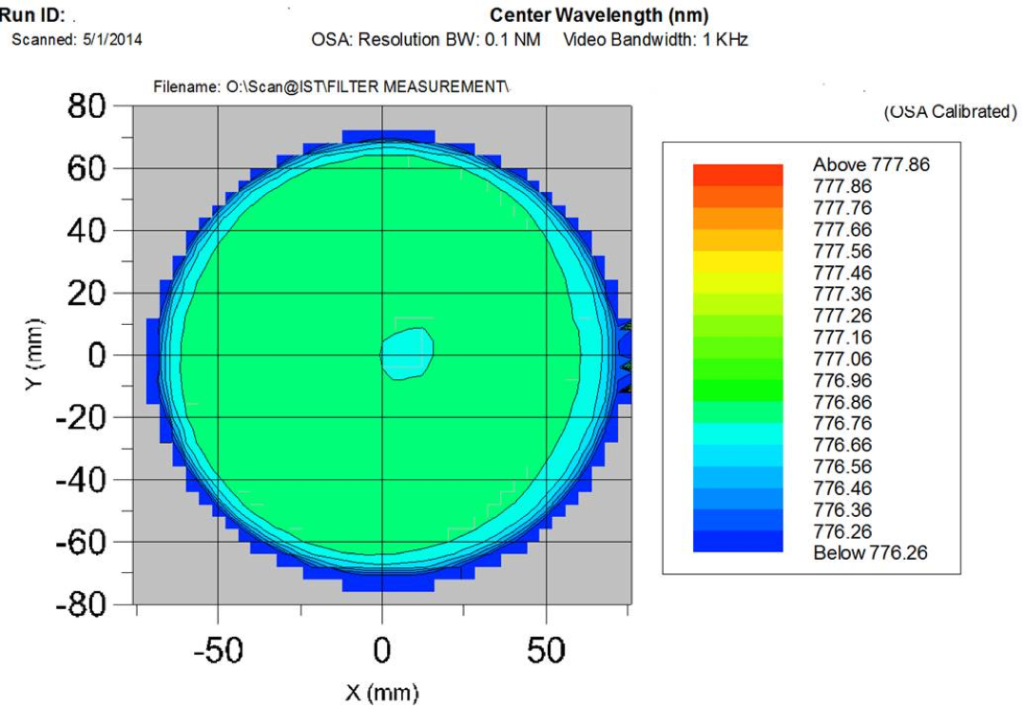
\includegraphics[scale=1.0]{imgs/barr_iridian.png}
\end{center}


De las mediciones del $17/9$, la banda verde tiene el siguiente espectro, parece ser bastante homogénea la banda, es decir que en cada punto x,y espacial de la banda el espectro de transmisión parece ser el mismo (esto habría que confirmarlo), se puede caracterizar con algún parámetro la homogeneidad del filtro? $\xrightarrow{}$ El objetivo de esta parte es lograr una buena \textsc{datasheet} del filtro.

\begin{center}
	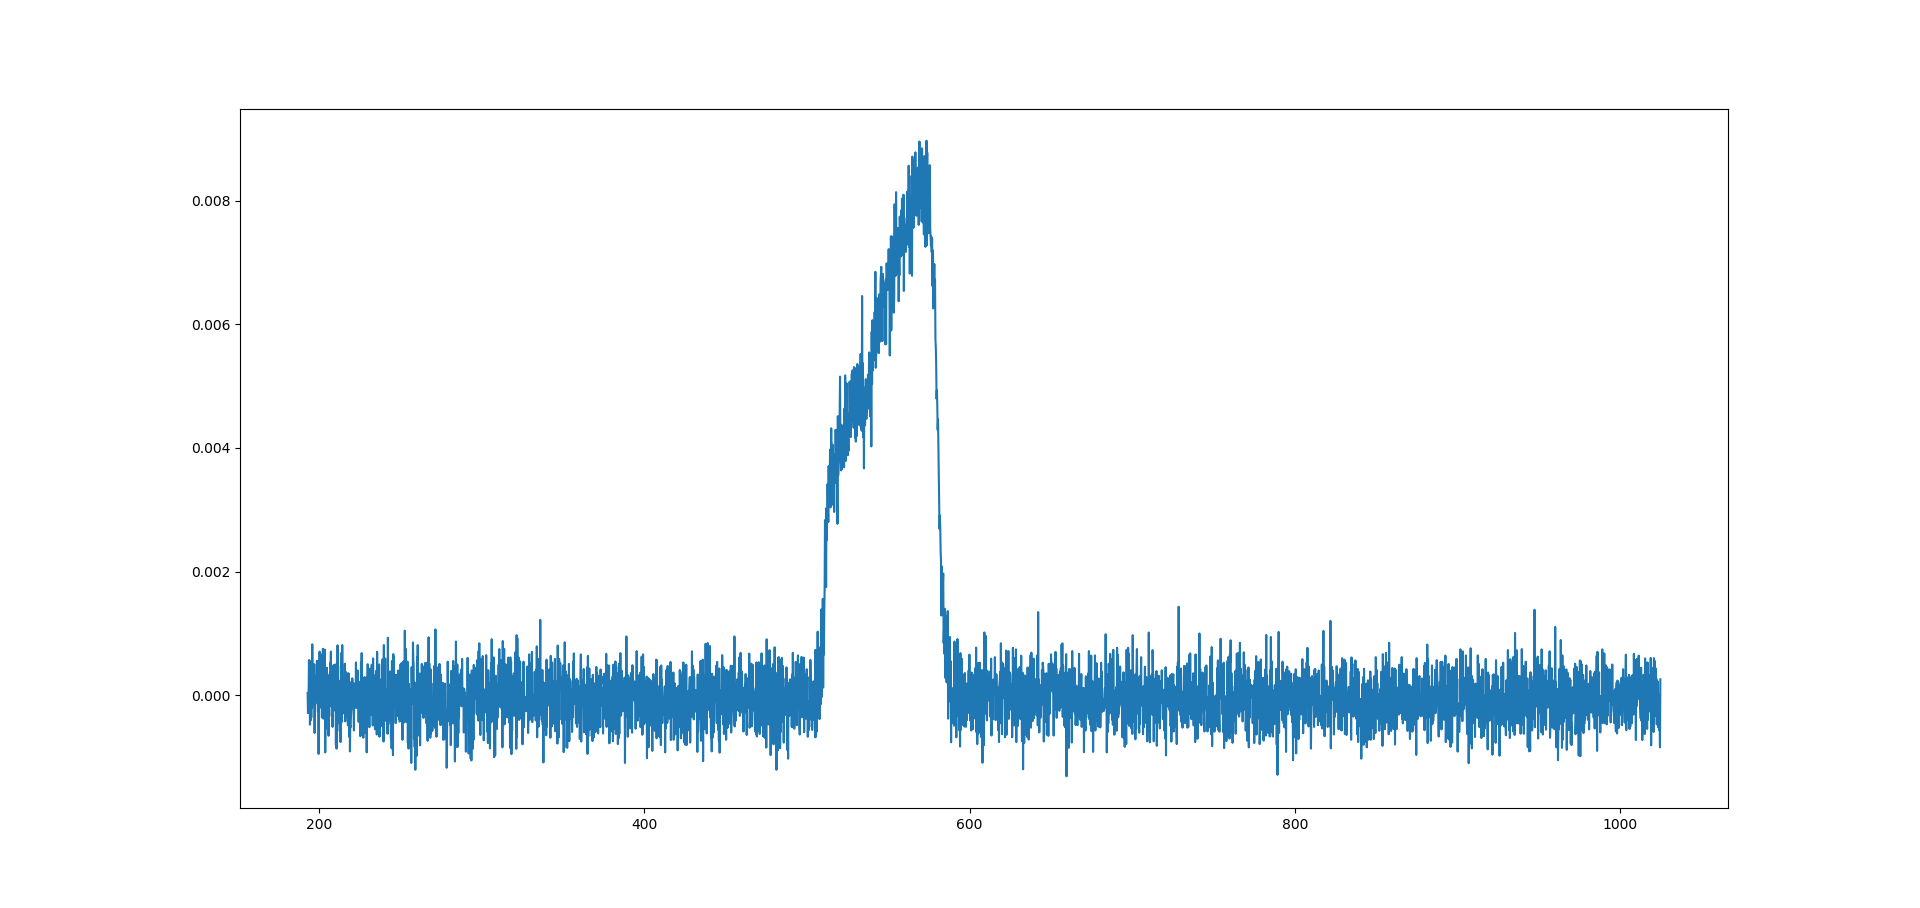
\includegraphics[scale=0.4]{imgs/green_band_spectra.png}
\end{center}


Ejemplo de datasheet del fabricante \textsc{Iridian}, sacado de \href{https://www.iridian.ca/product/bpf-9460-180/}{aquí}:

\begin{center}
	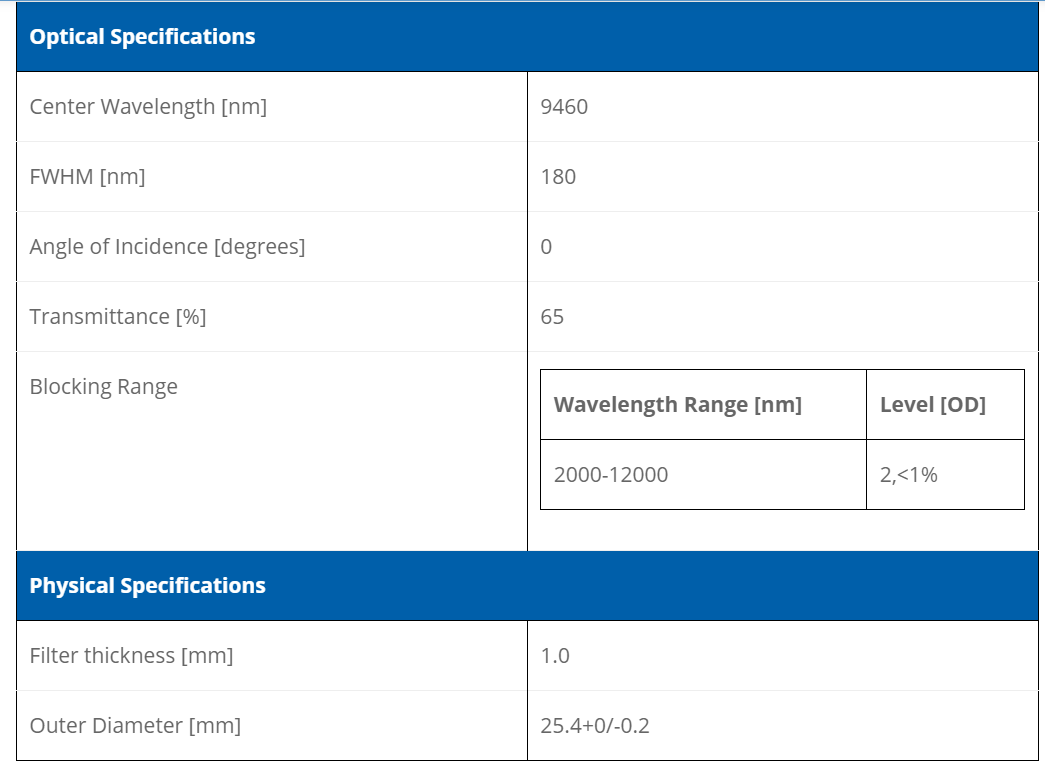
\includegraphics[scale=0.8]{imgs/datasheet_modelo.png}
\end{center}

Mediciones espectrómetro son de intensidad.. queremos transmisión.

Canal copado de repaso de cosas de óptica: \href{https://www.youtube.com/user/kridnix/videos}{kridnix}

\newpage
\hrulefill

$23/9/2019$

Ya me imprimieron la pieza, gracias Hilario! (por buscarmela antes de que se vayan los del taller).


\hrulefill

$25/9/2019$

mediciones de hoy.. 

$\Delta x = \Delta y = 13 mm$, pasos de 500 $\mu m$ en la 1era medición y de 10 $\mu m$ en la 2da medición.

Fuente de luz utilizada: \texttt{Fiber-Lite 190 Illuminator, 30 watt Halogen light source w/ EKZ lamp}, link: \url{https://dolan-jenner.com/products/fiber-lite-190}

\texttt{datasheet}: \url{https://www.setra.com/hubfs/products/illuminators/model-190-data-sheet.pdf}


\hrulefill

$27/9/2019$

apróx 18hs tarda un barrido de 13mm x 13 mm con un paso de 50 micrones tanto en dx como en dy.

Algunas fotos del setup del barrido:

\begin{center}
	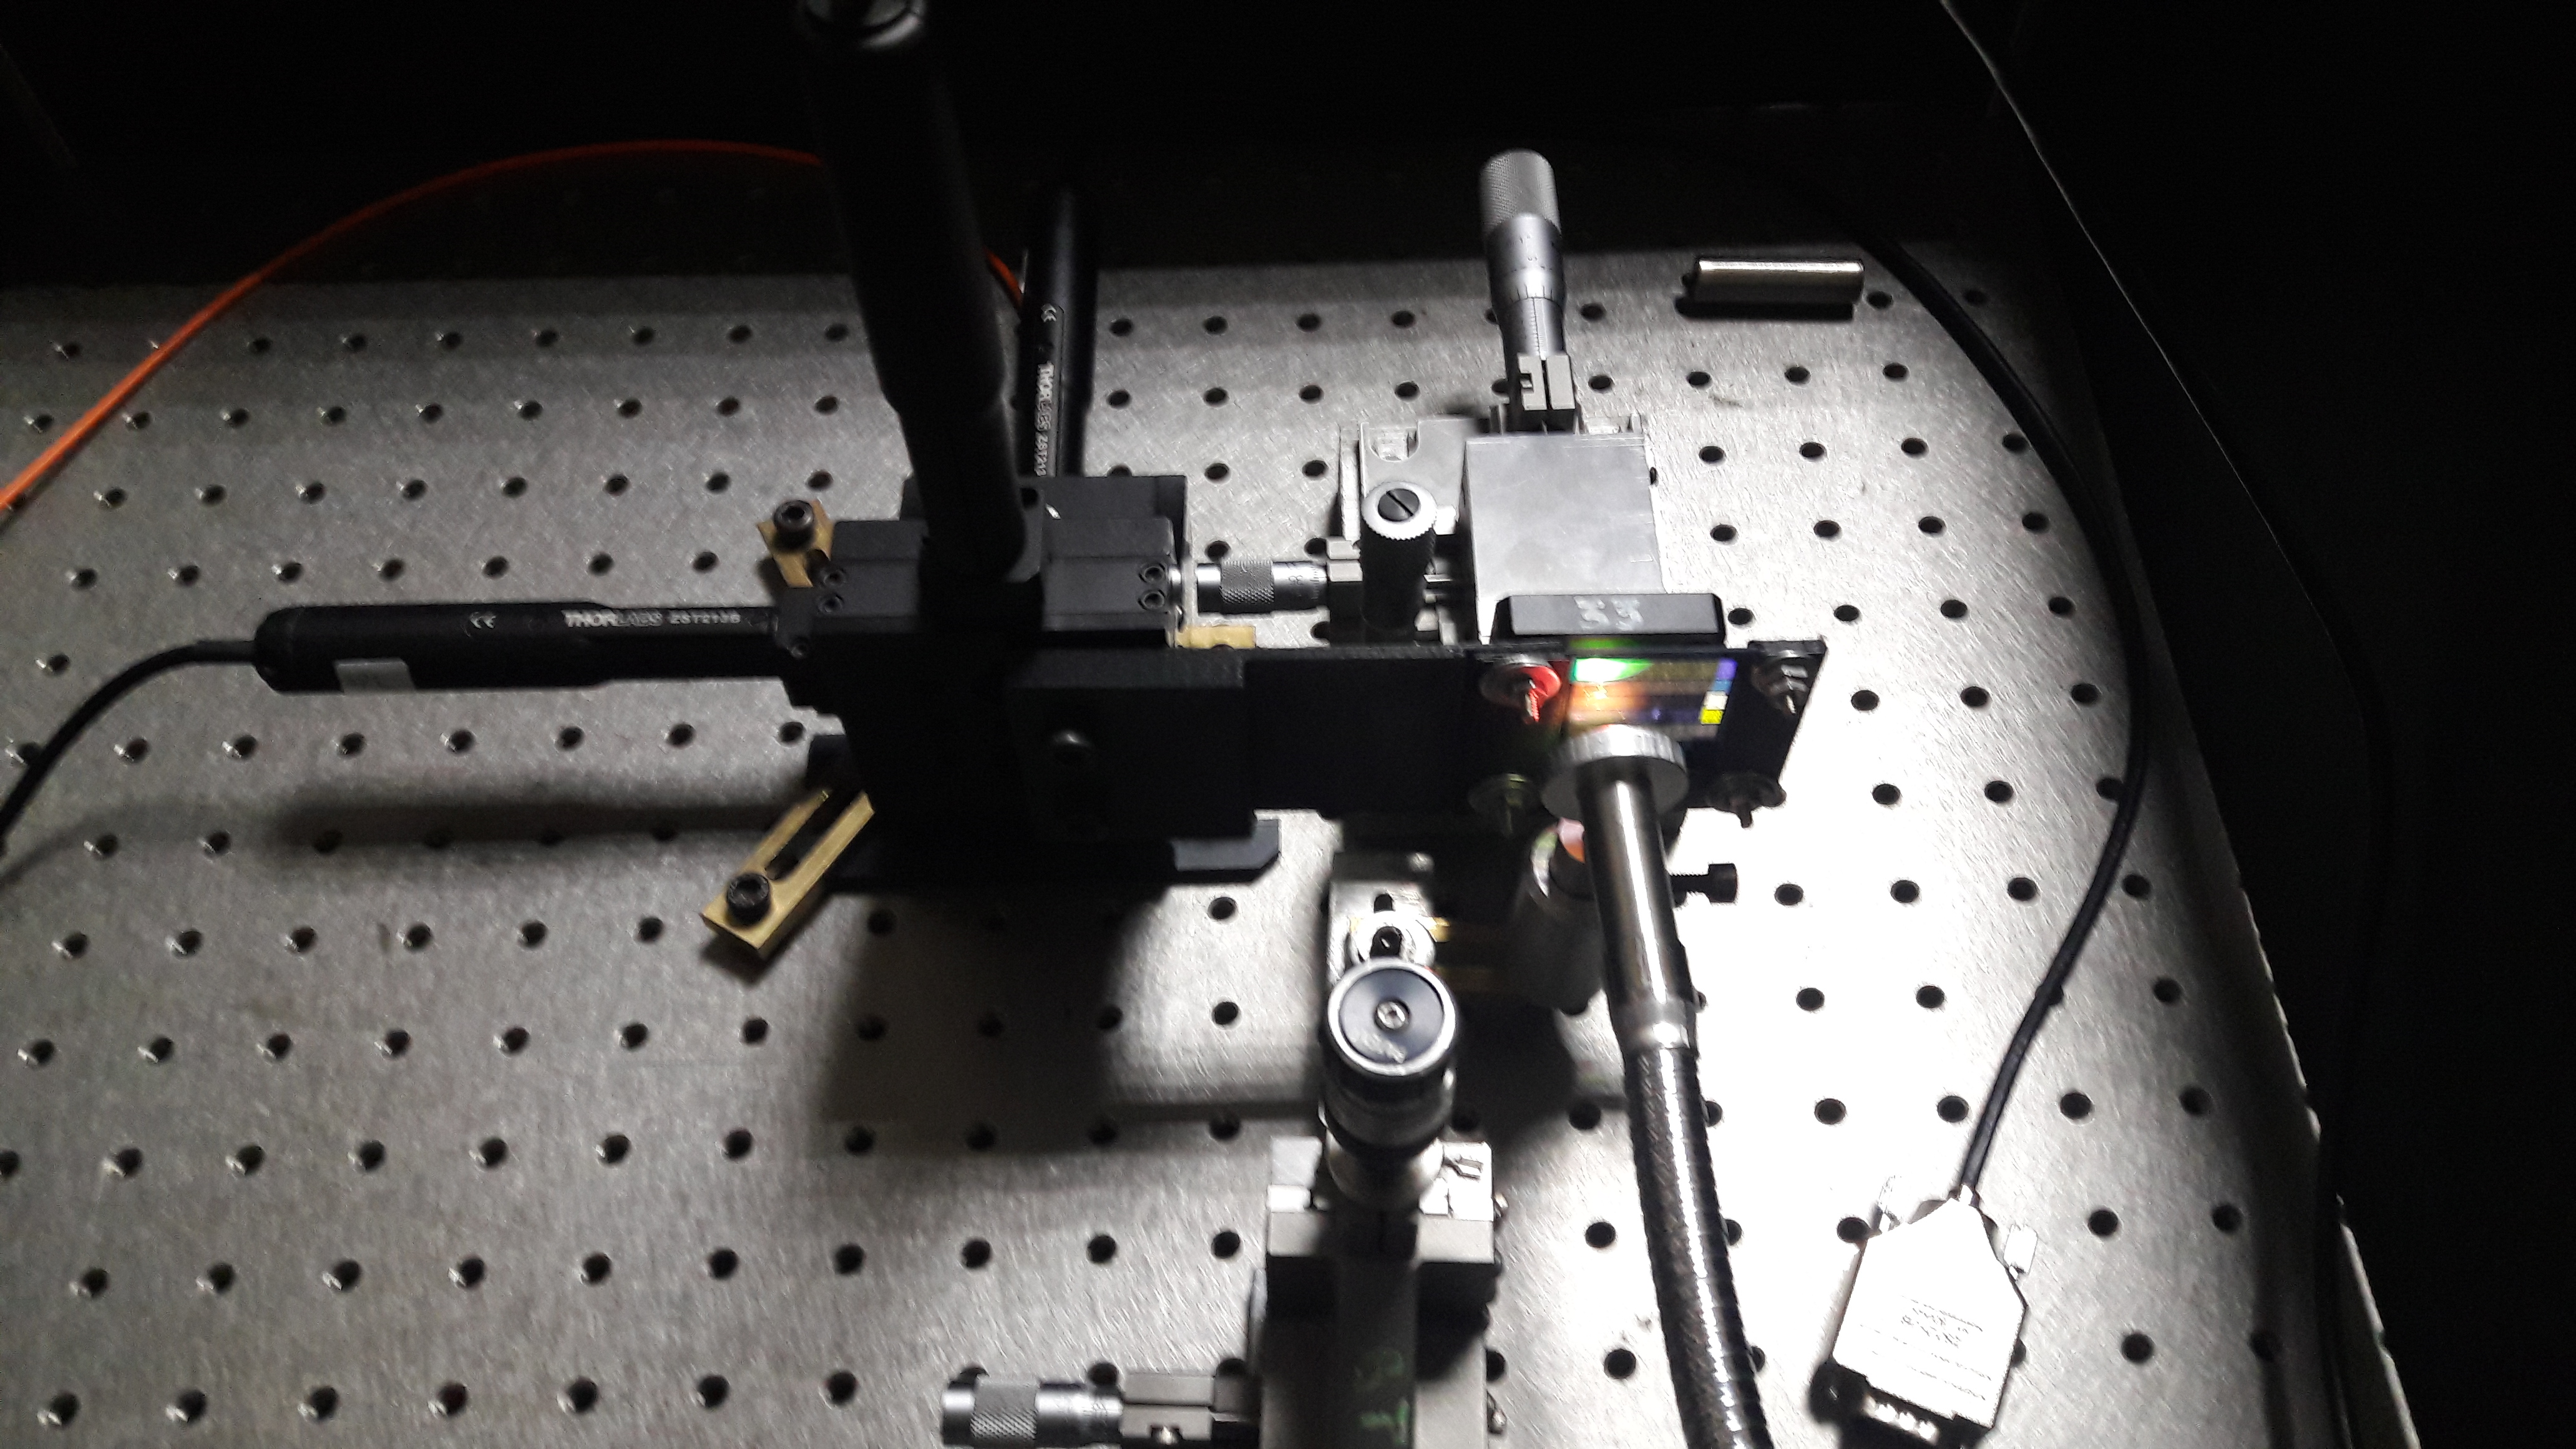
\includegraphics[scale=0.1]{imgs/setup_barrido/1.jpg}
\end{center}

\begin{center}
	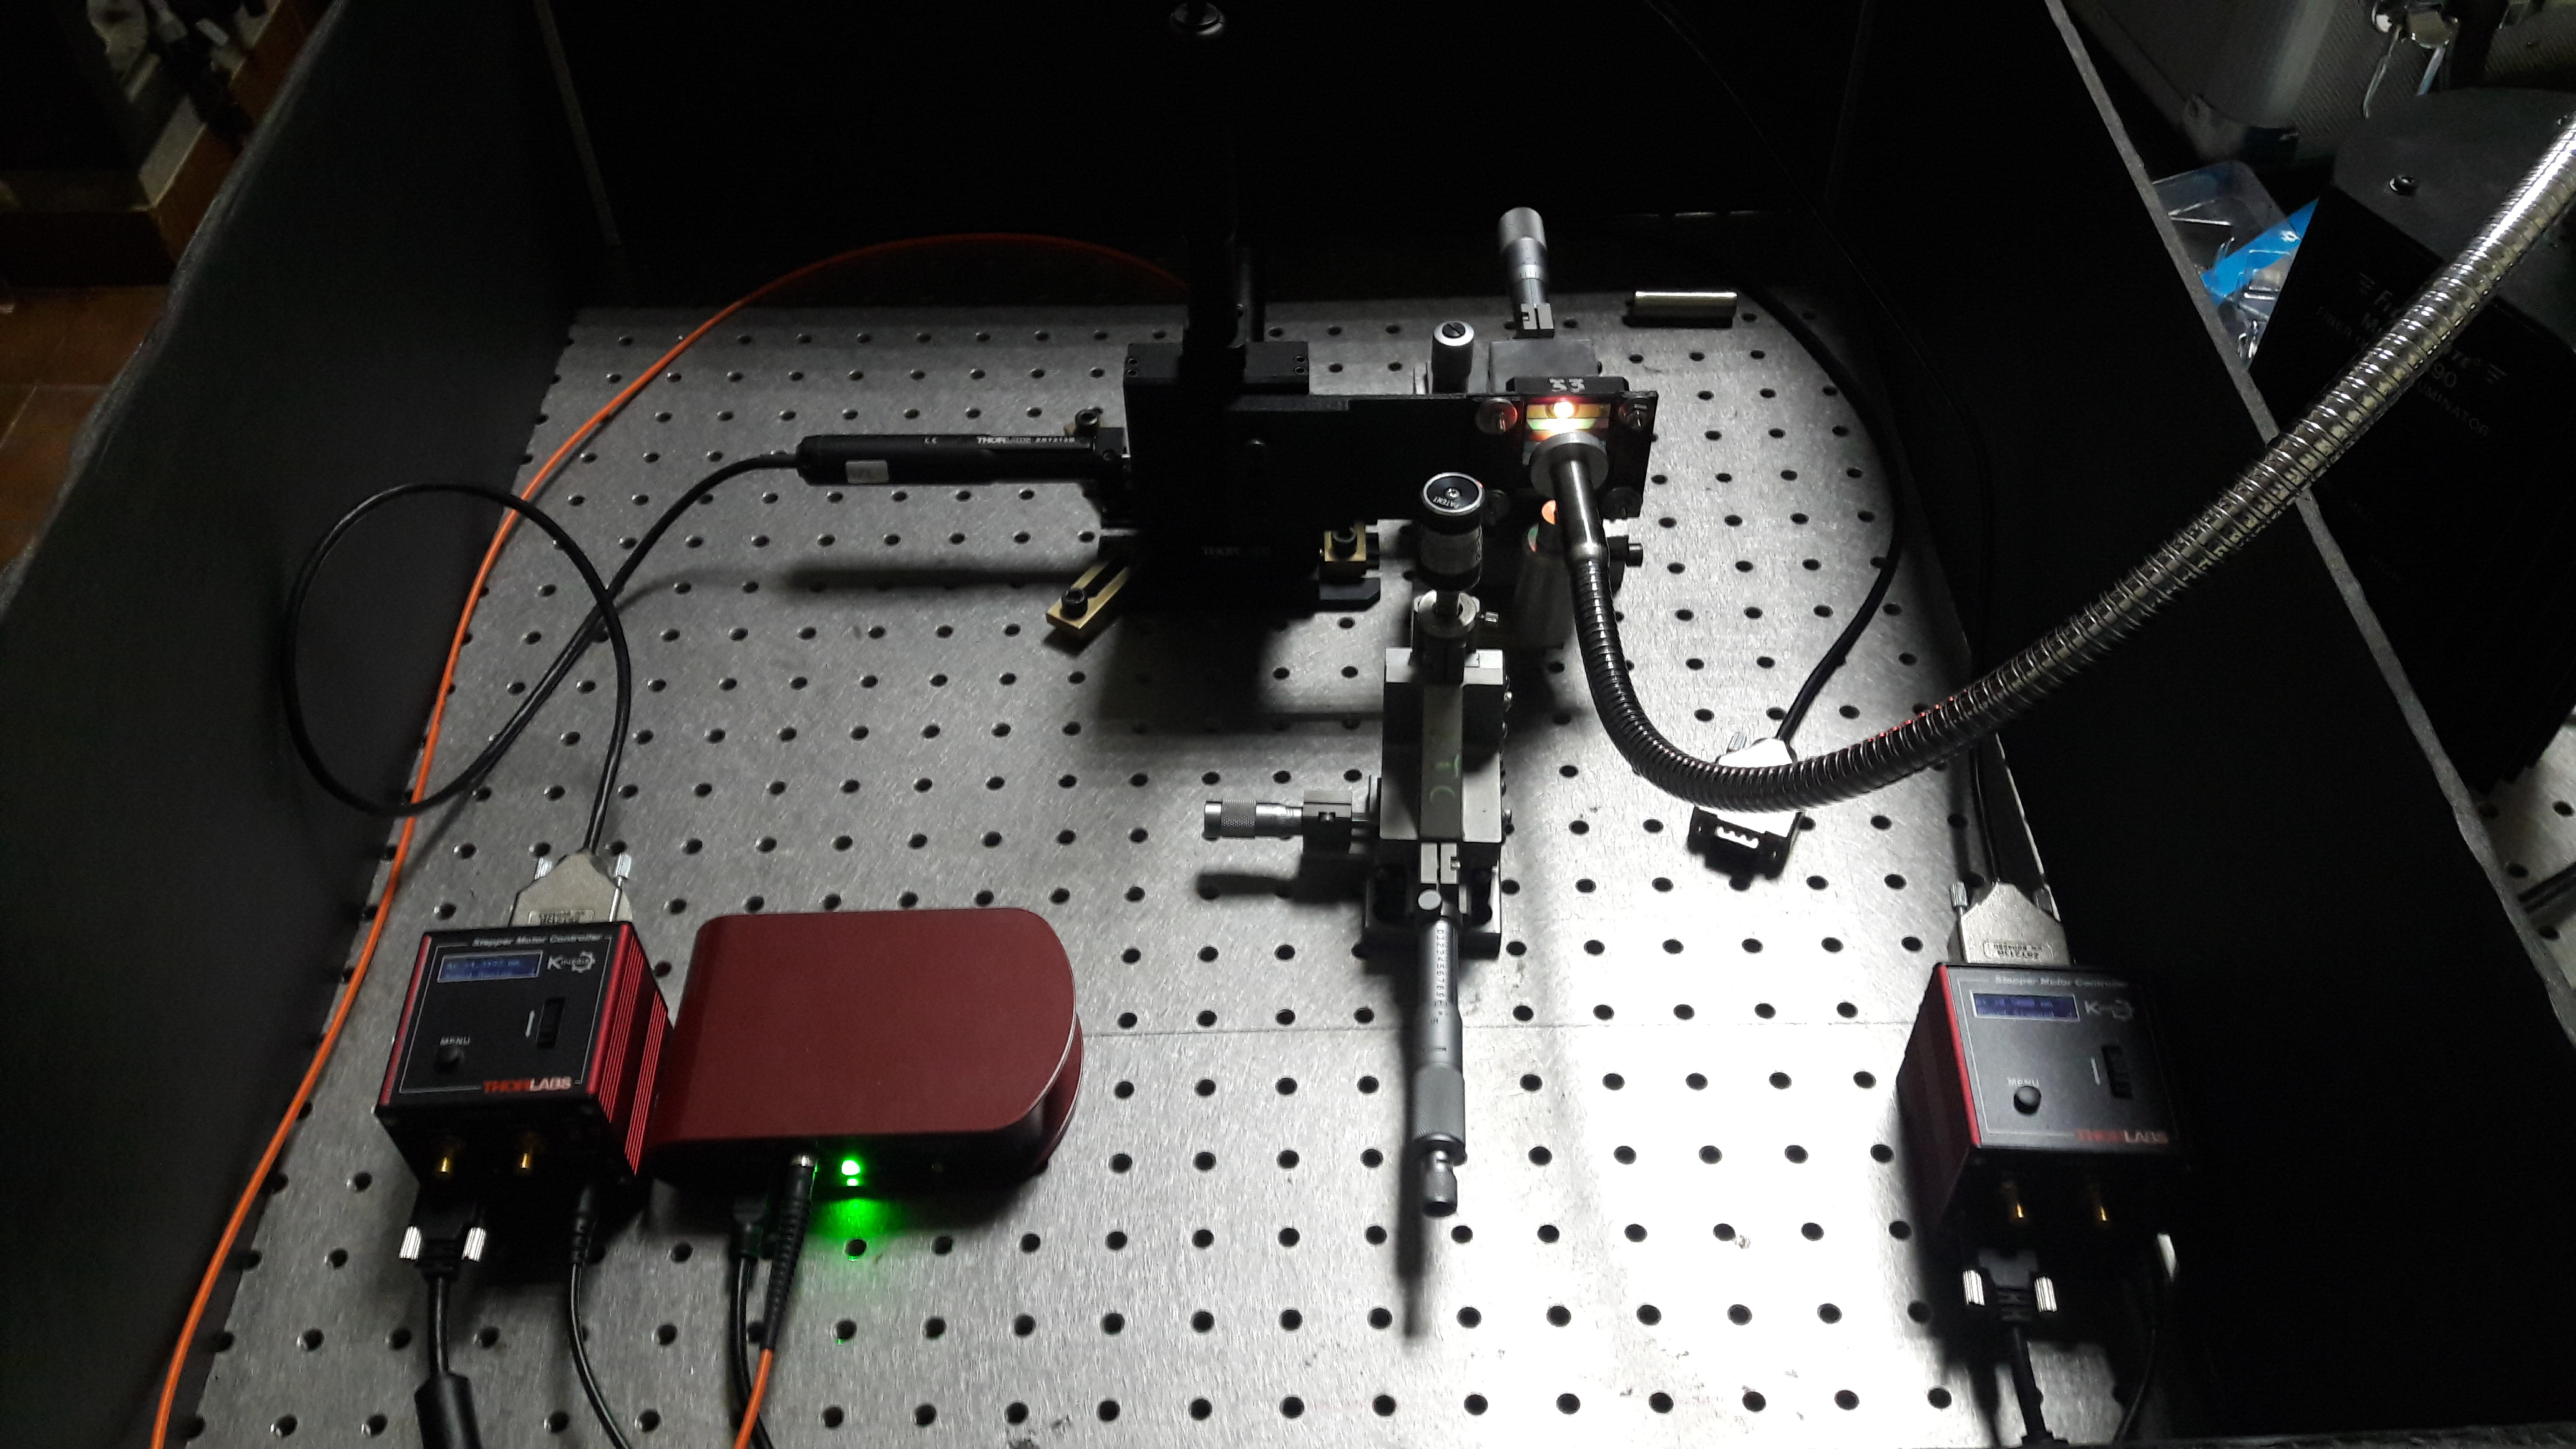
\includegraphics[scale=0.1]{imgs/setup_barrido/2.jpg}
\end{center}

\begin{center}
	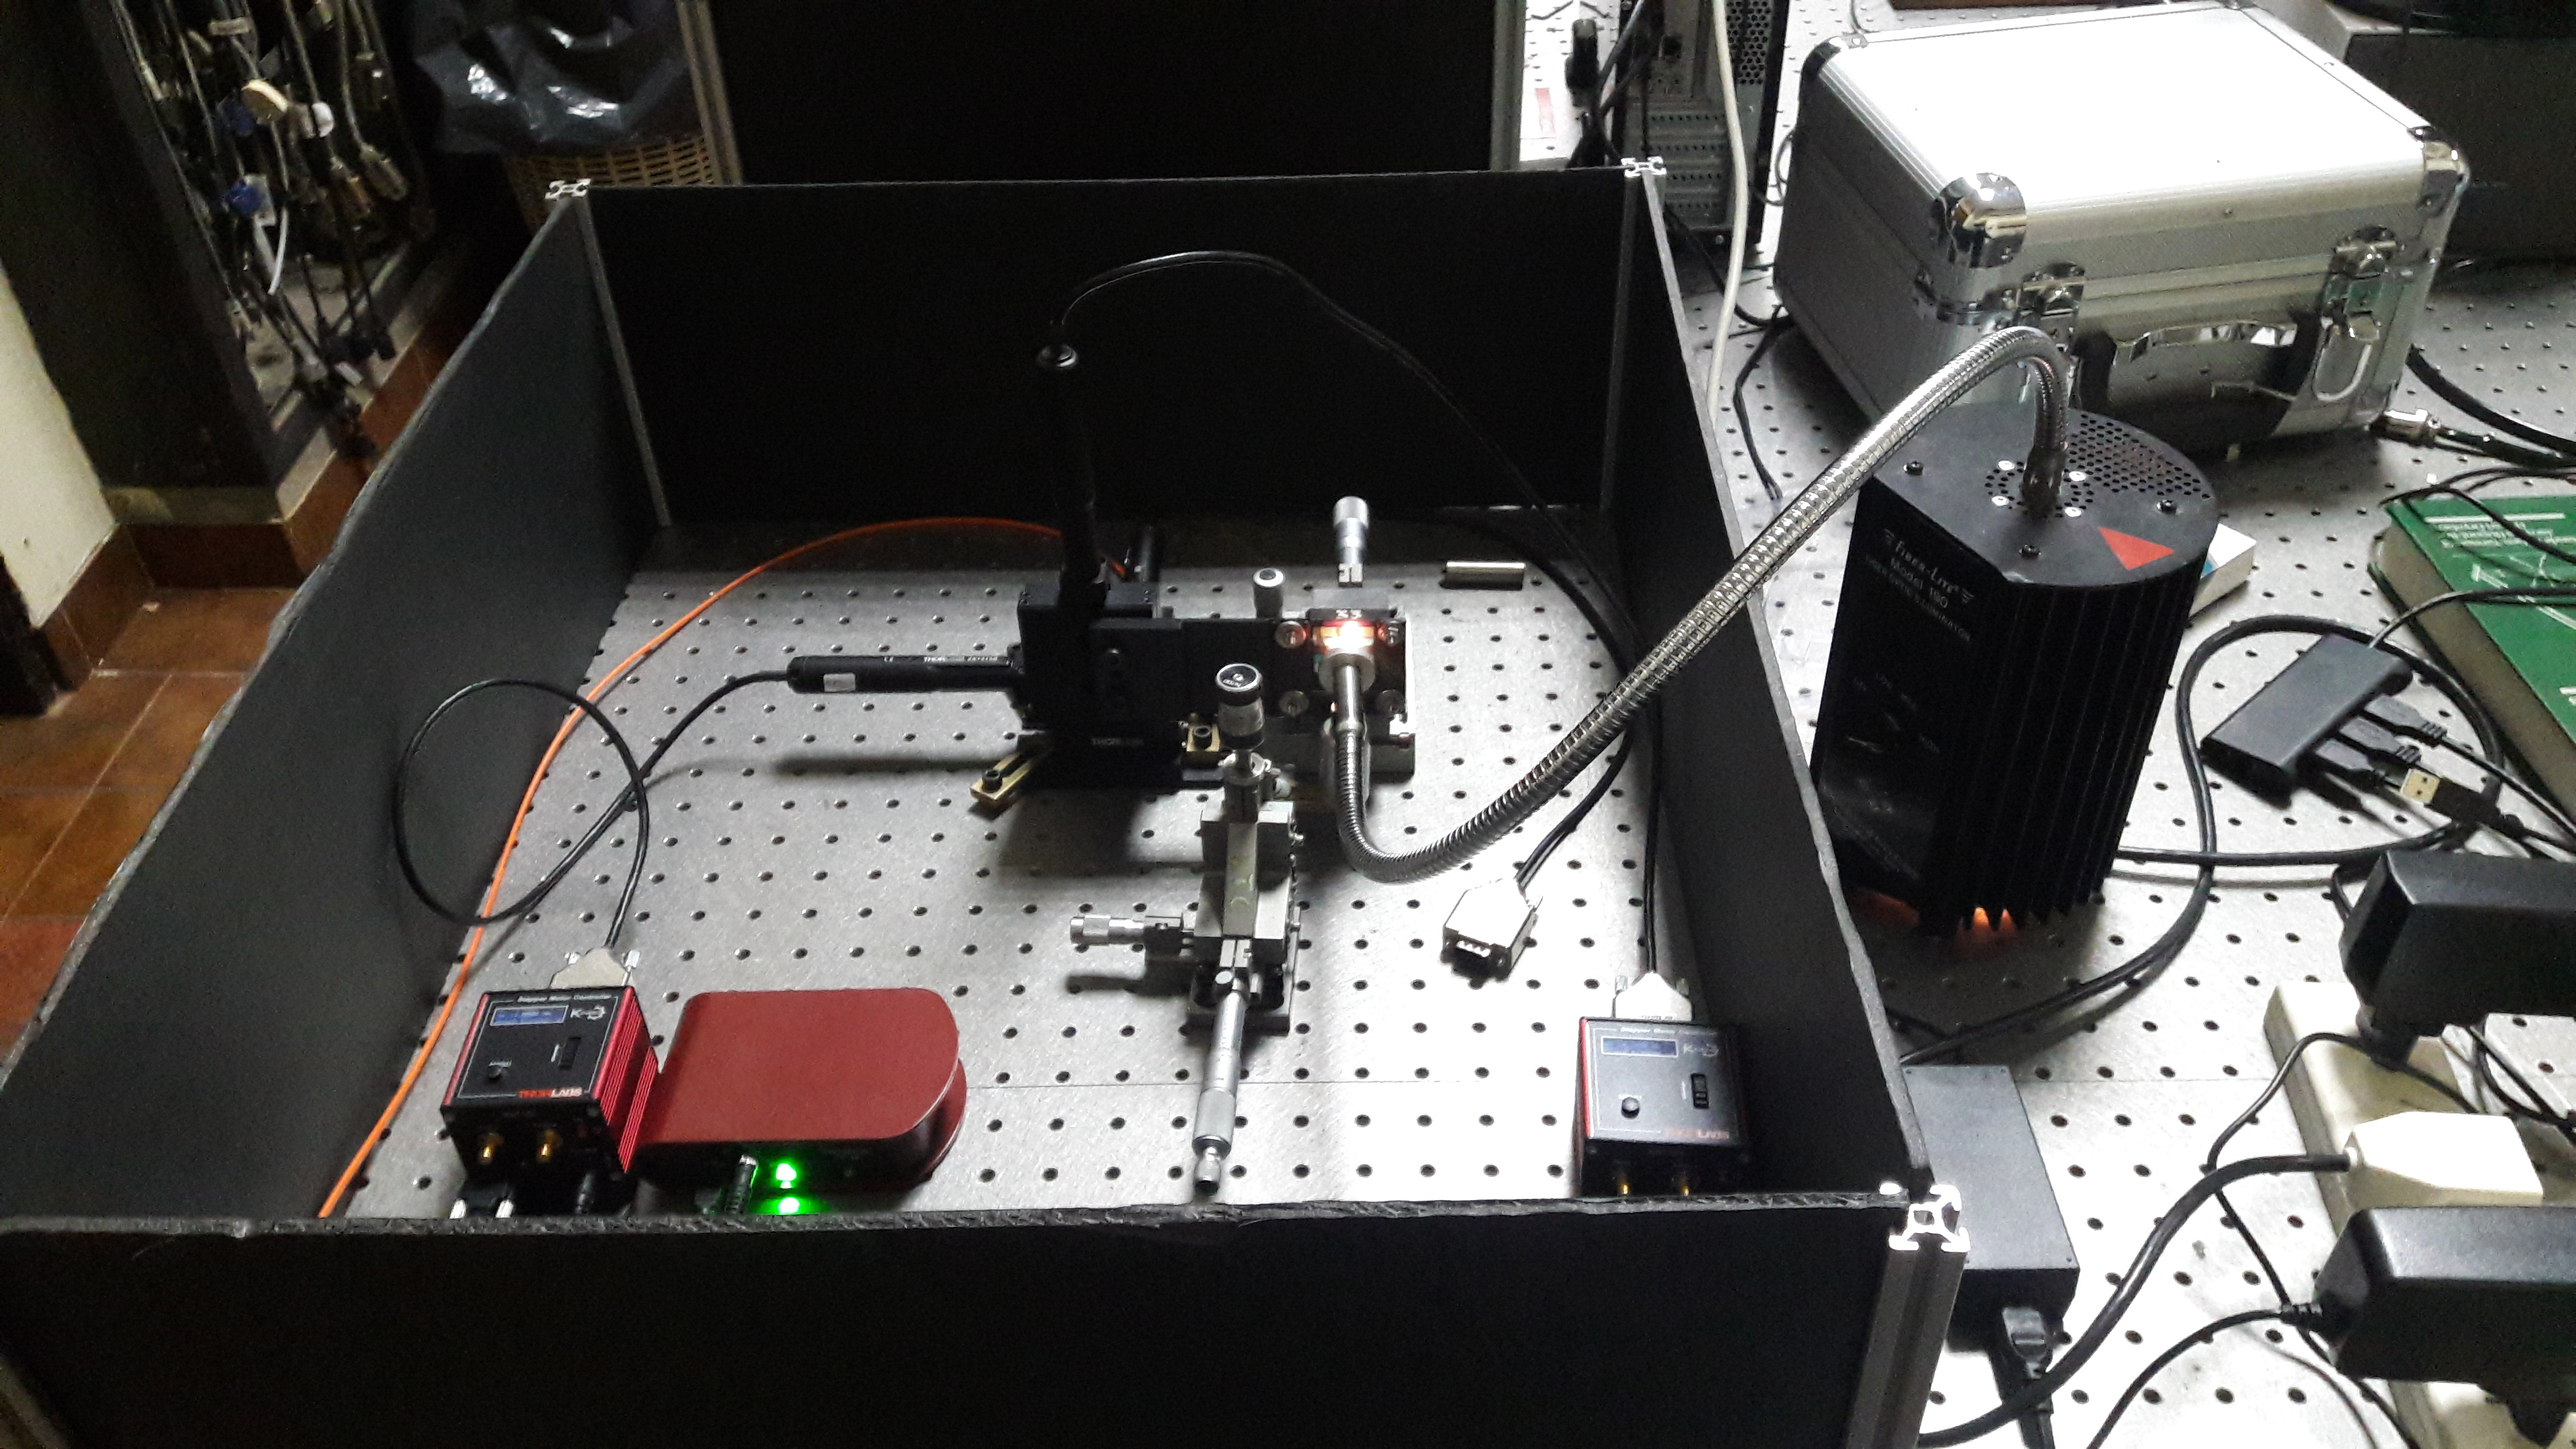
\includegraphics[scale=0.1]{imgs/setup_barrido/3.jpg}
\end{center}

\begin{center}
	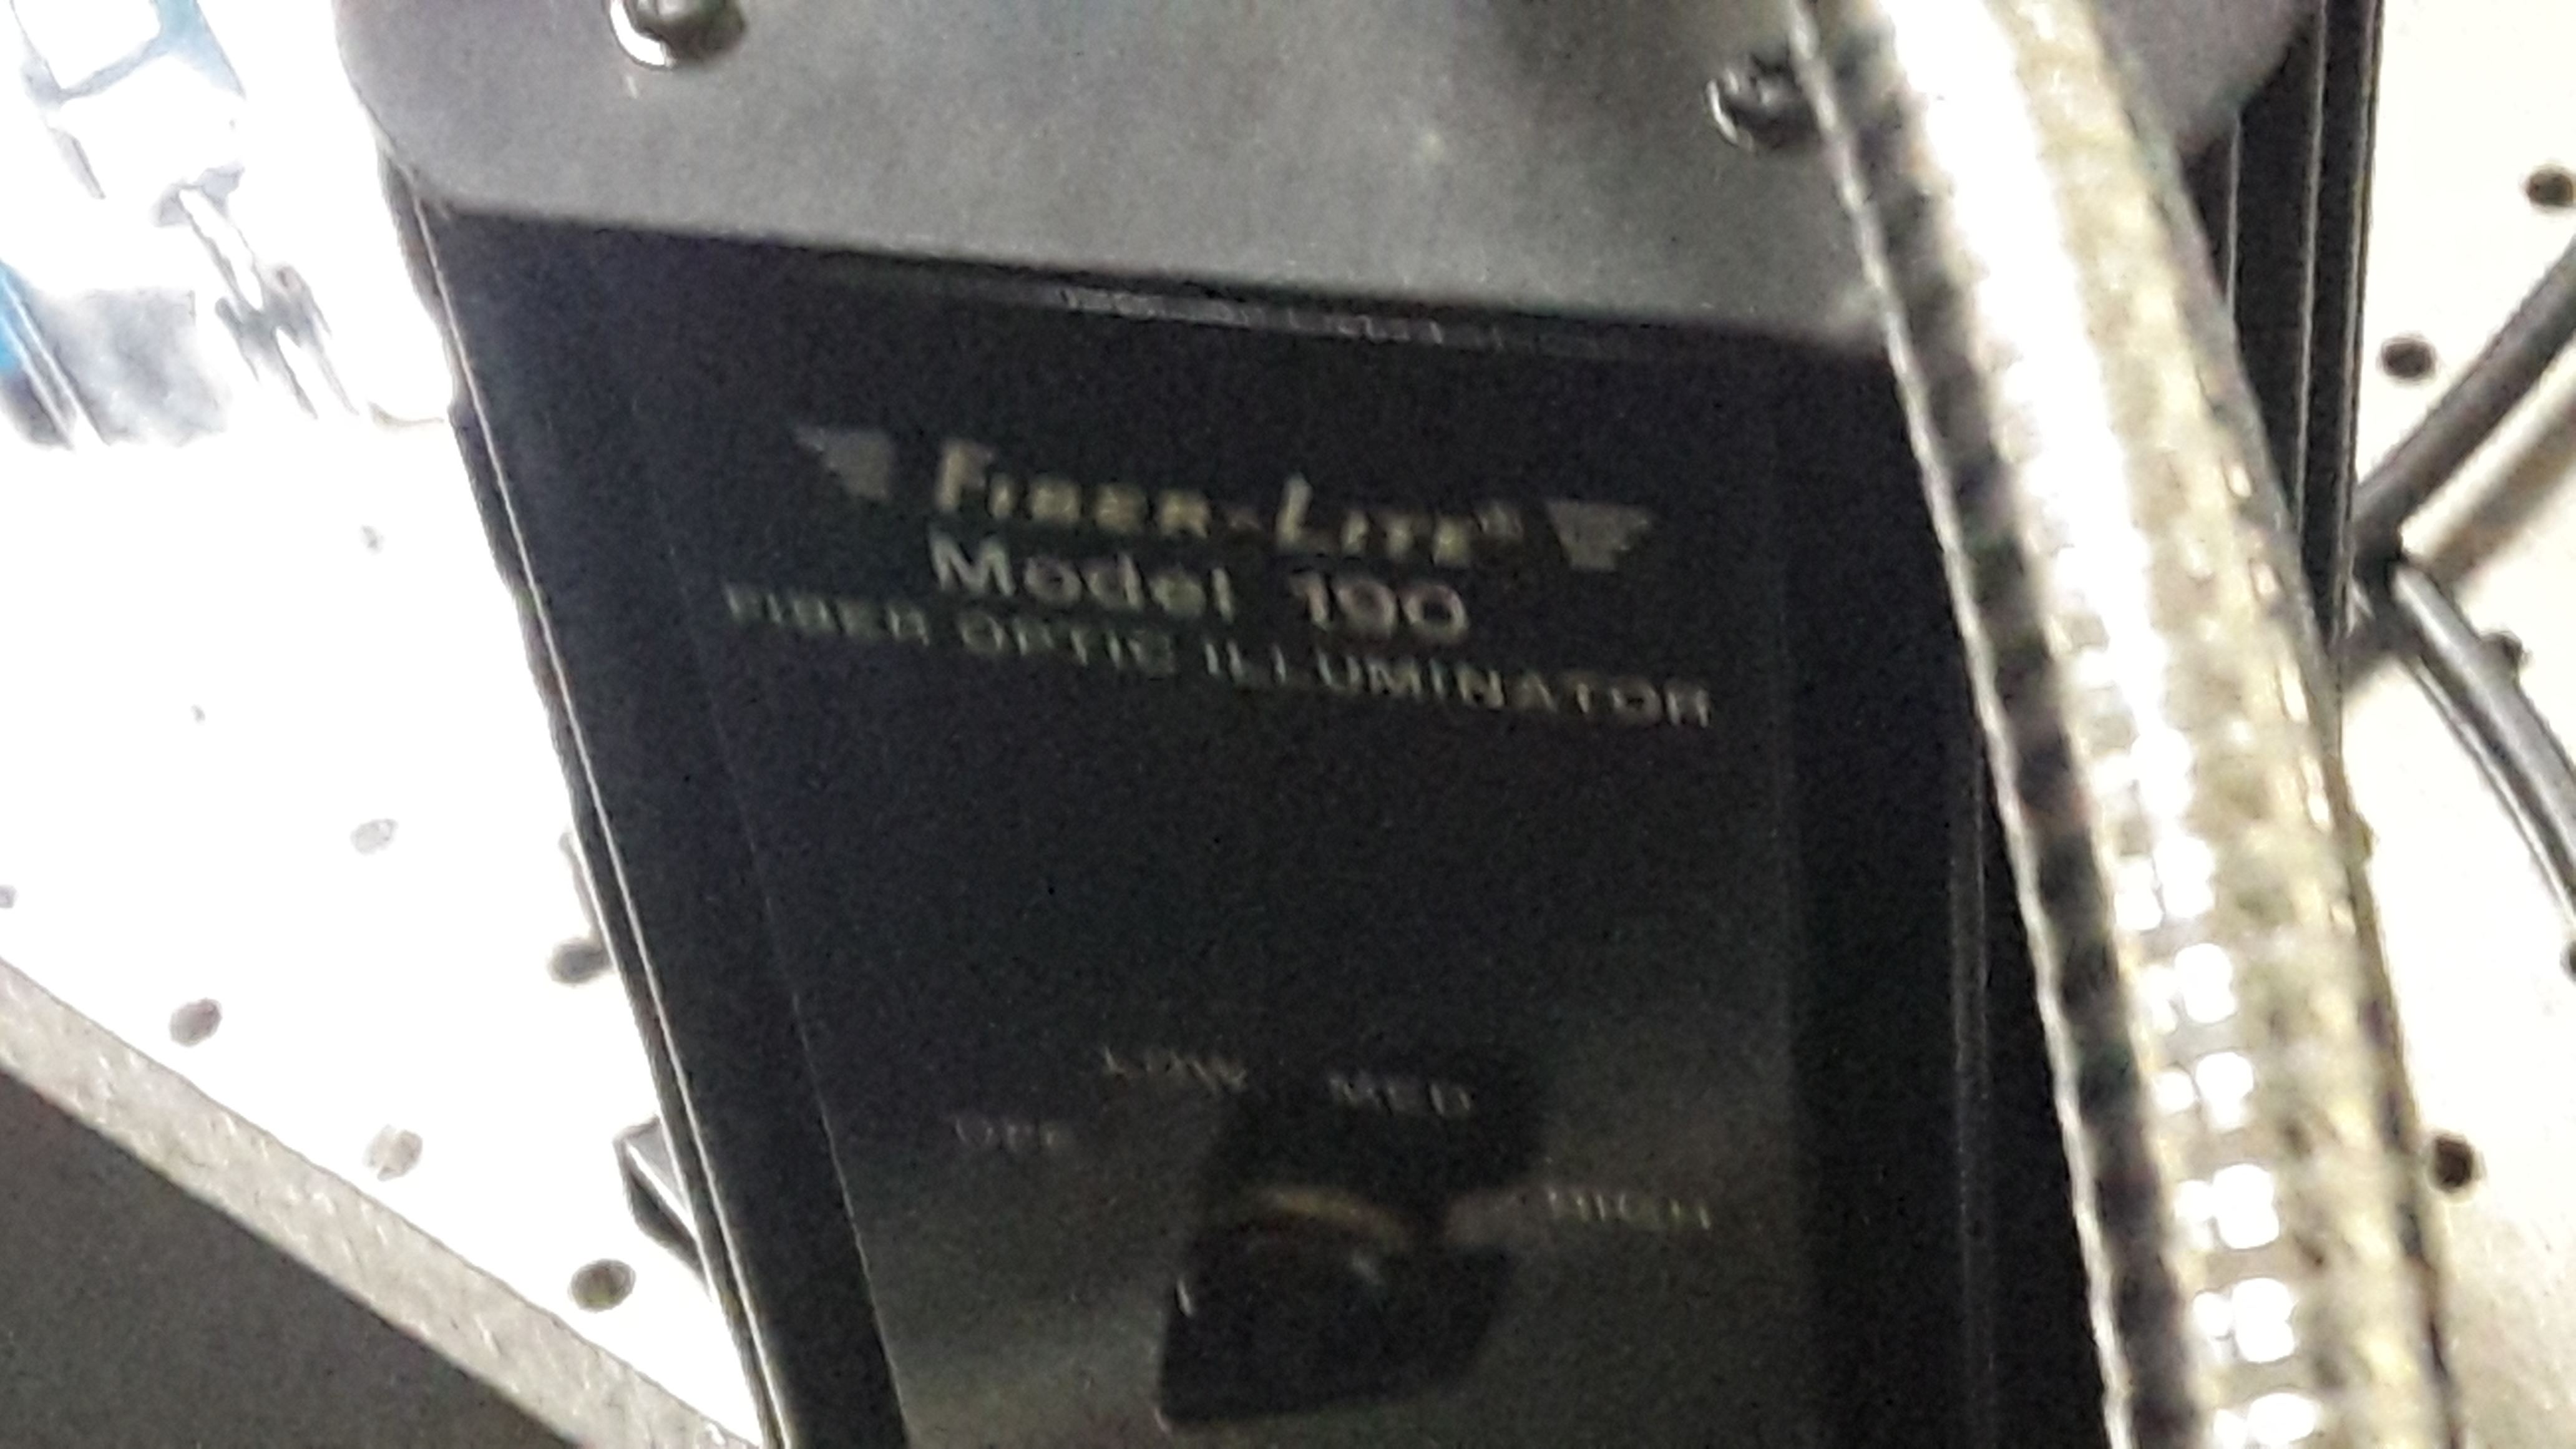
\includegraphics[scale=0.1]{imgs/setup_barrido/4.jpg}
\end{center}

\begin{center}
	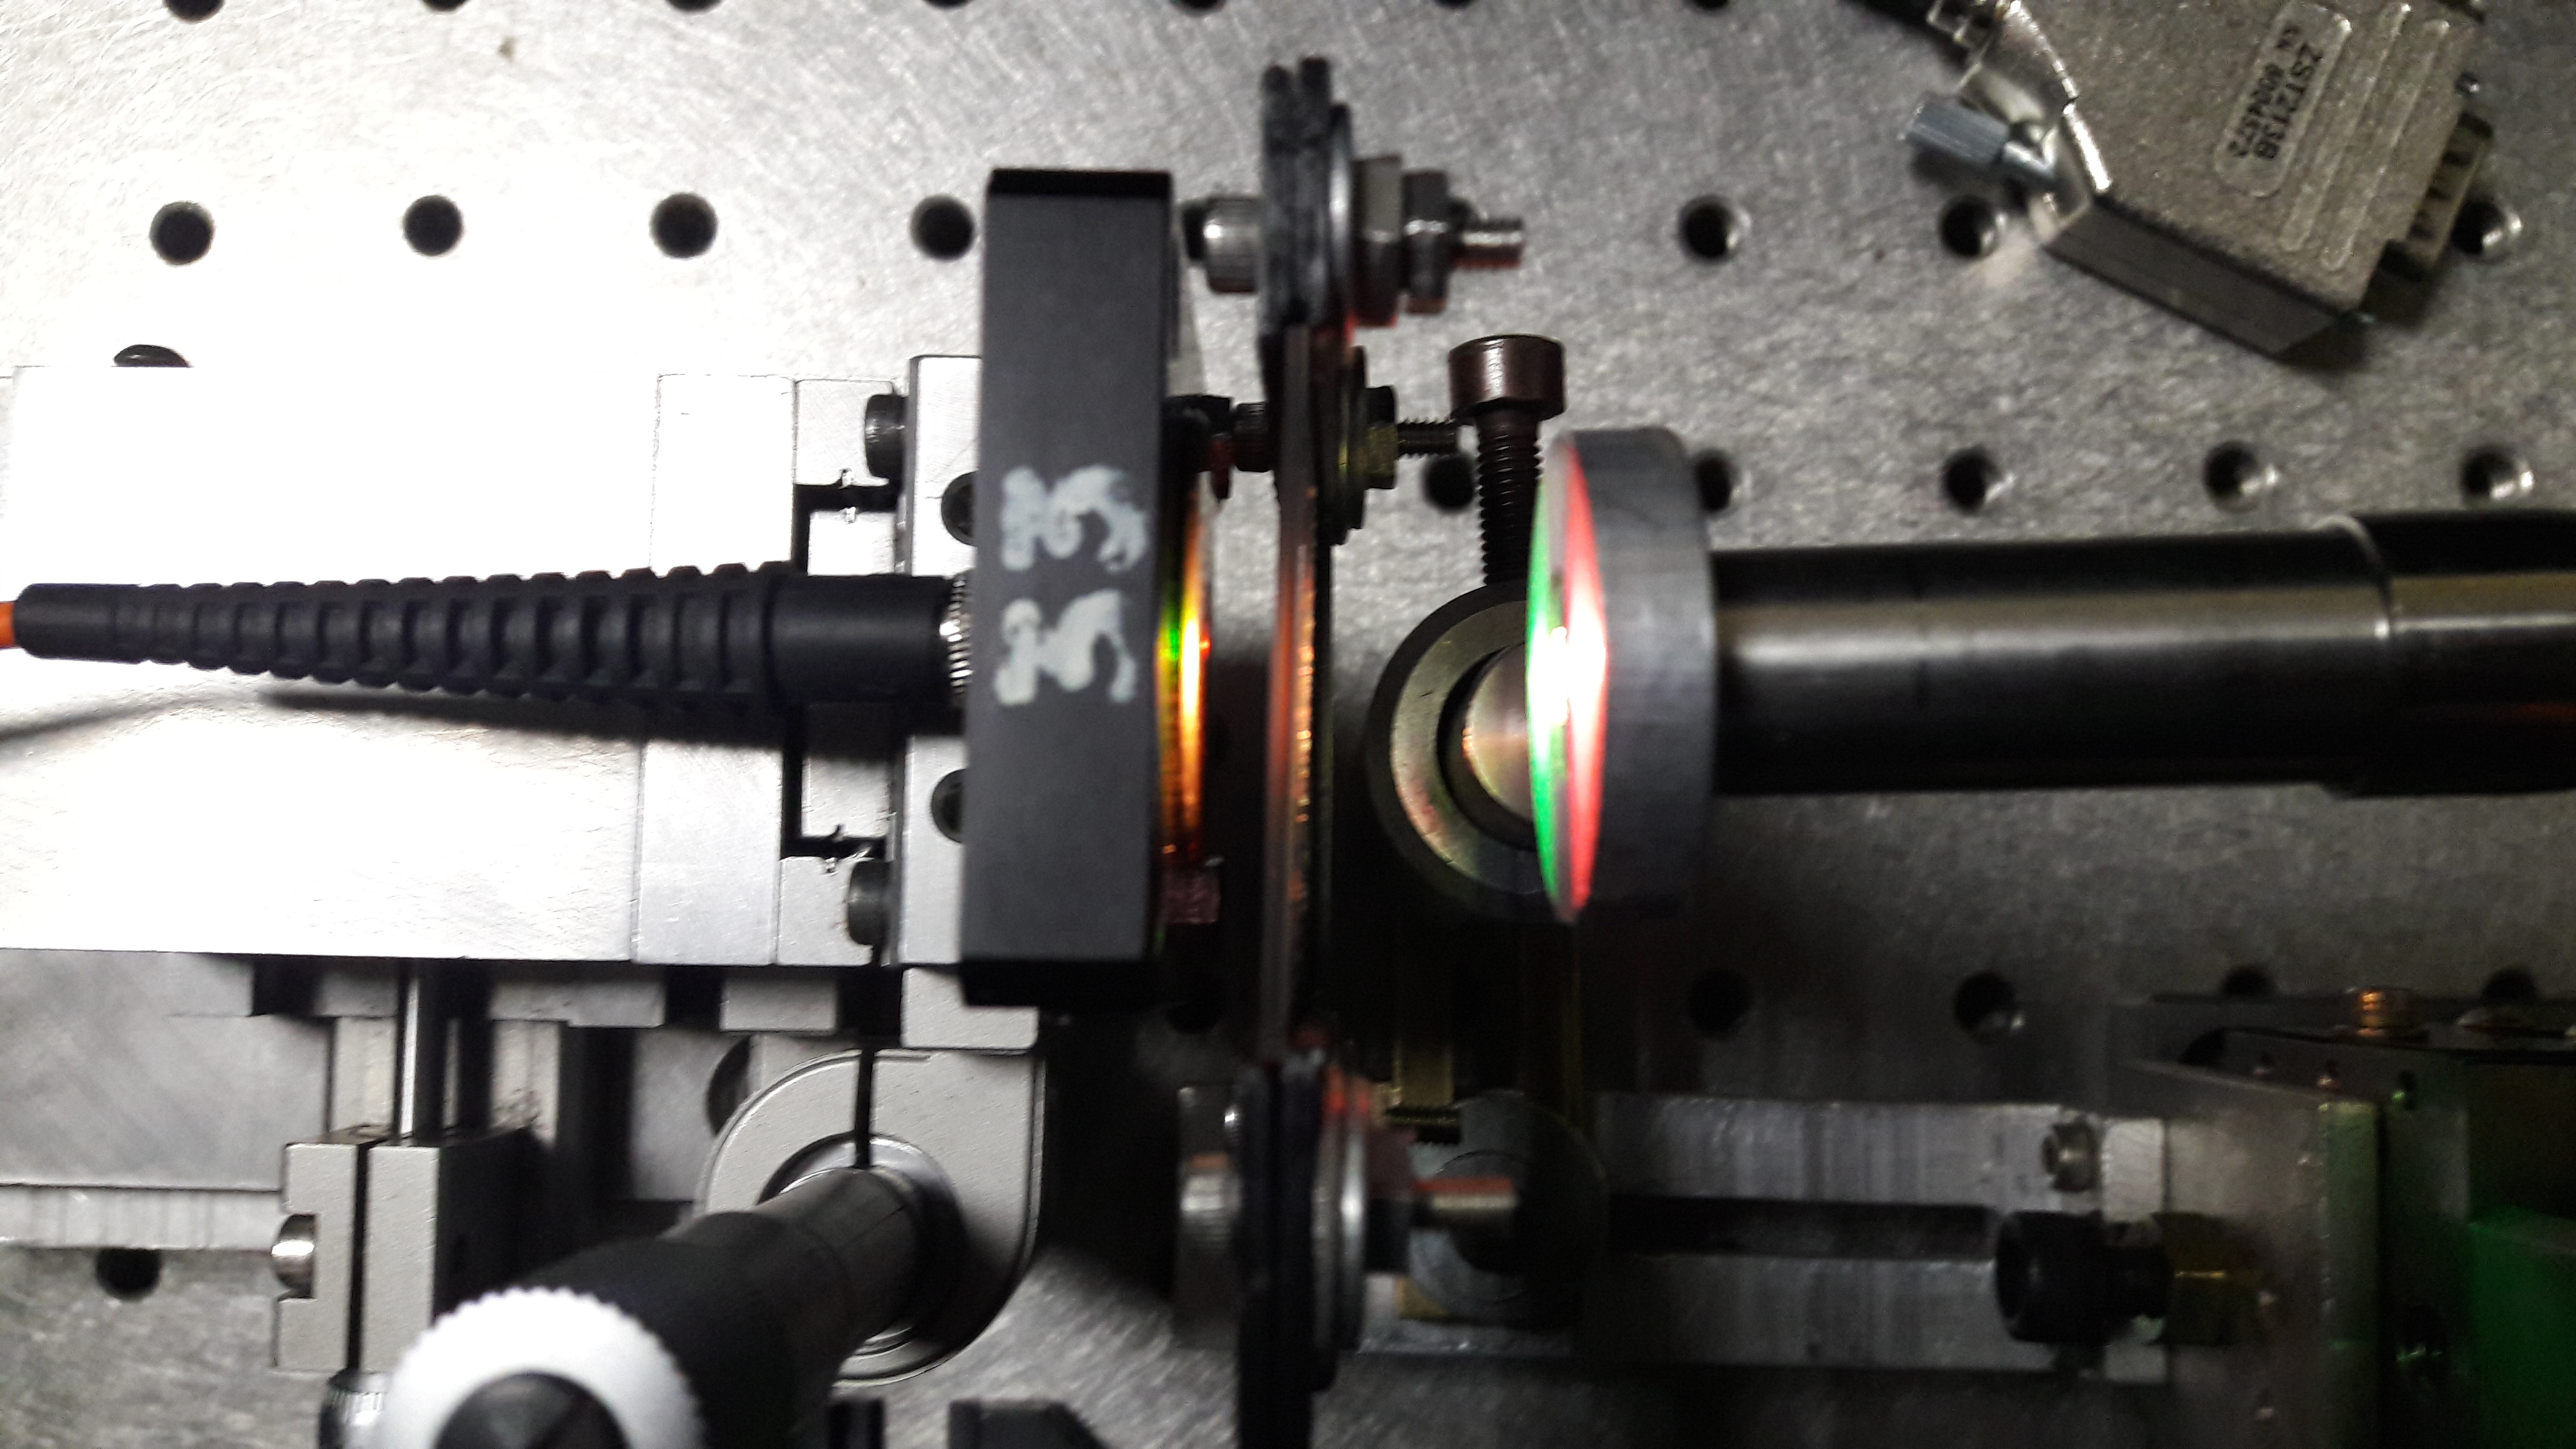
\includegraphics[scale=0.1]{imgs/setup_barrido/5.jpg}
\end{center}

\begin{center}
	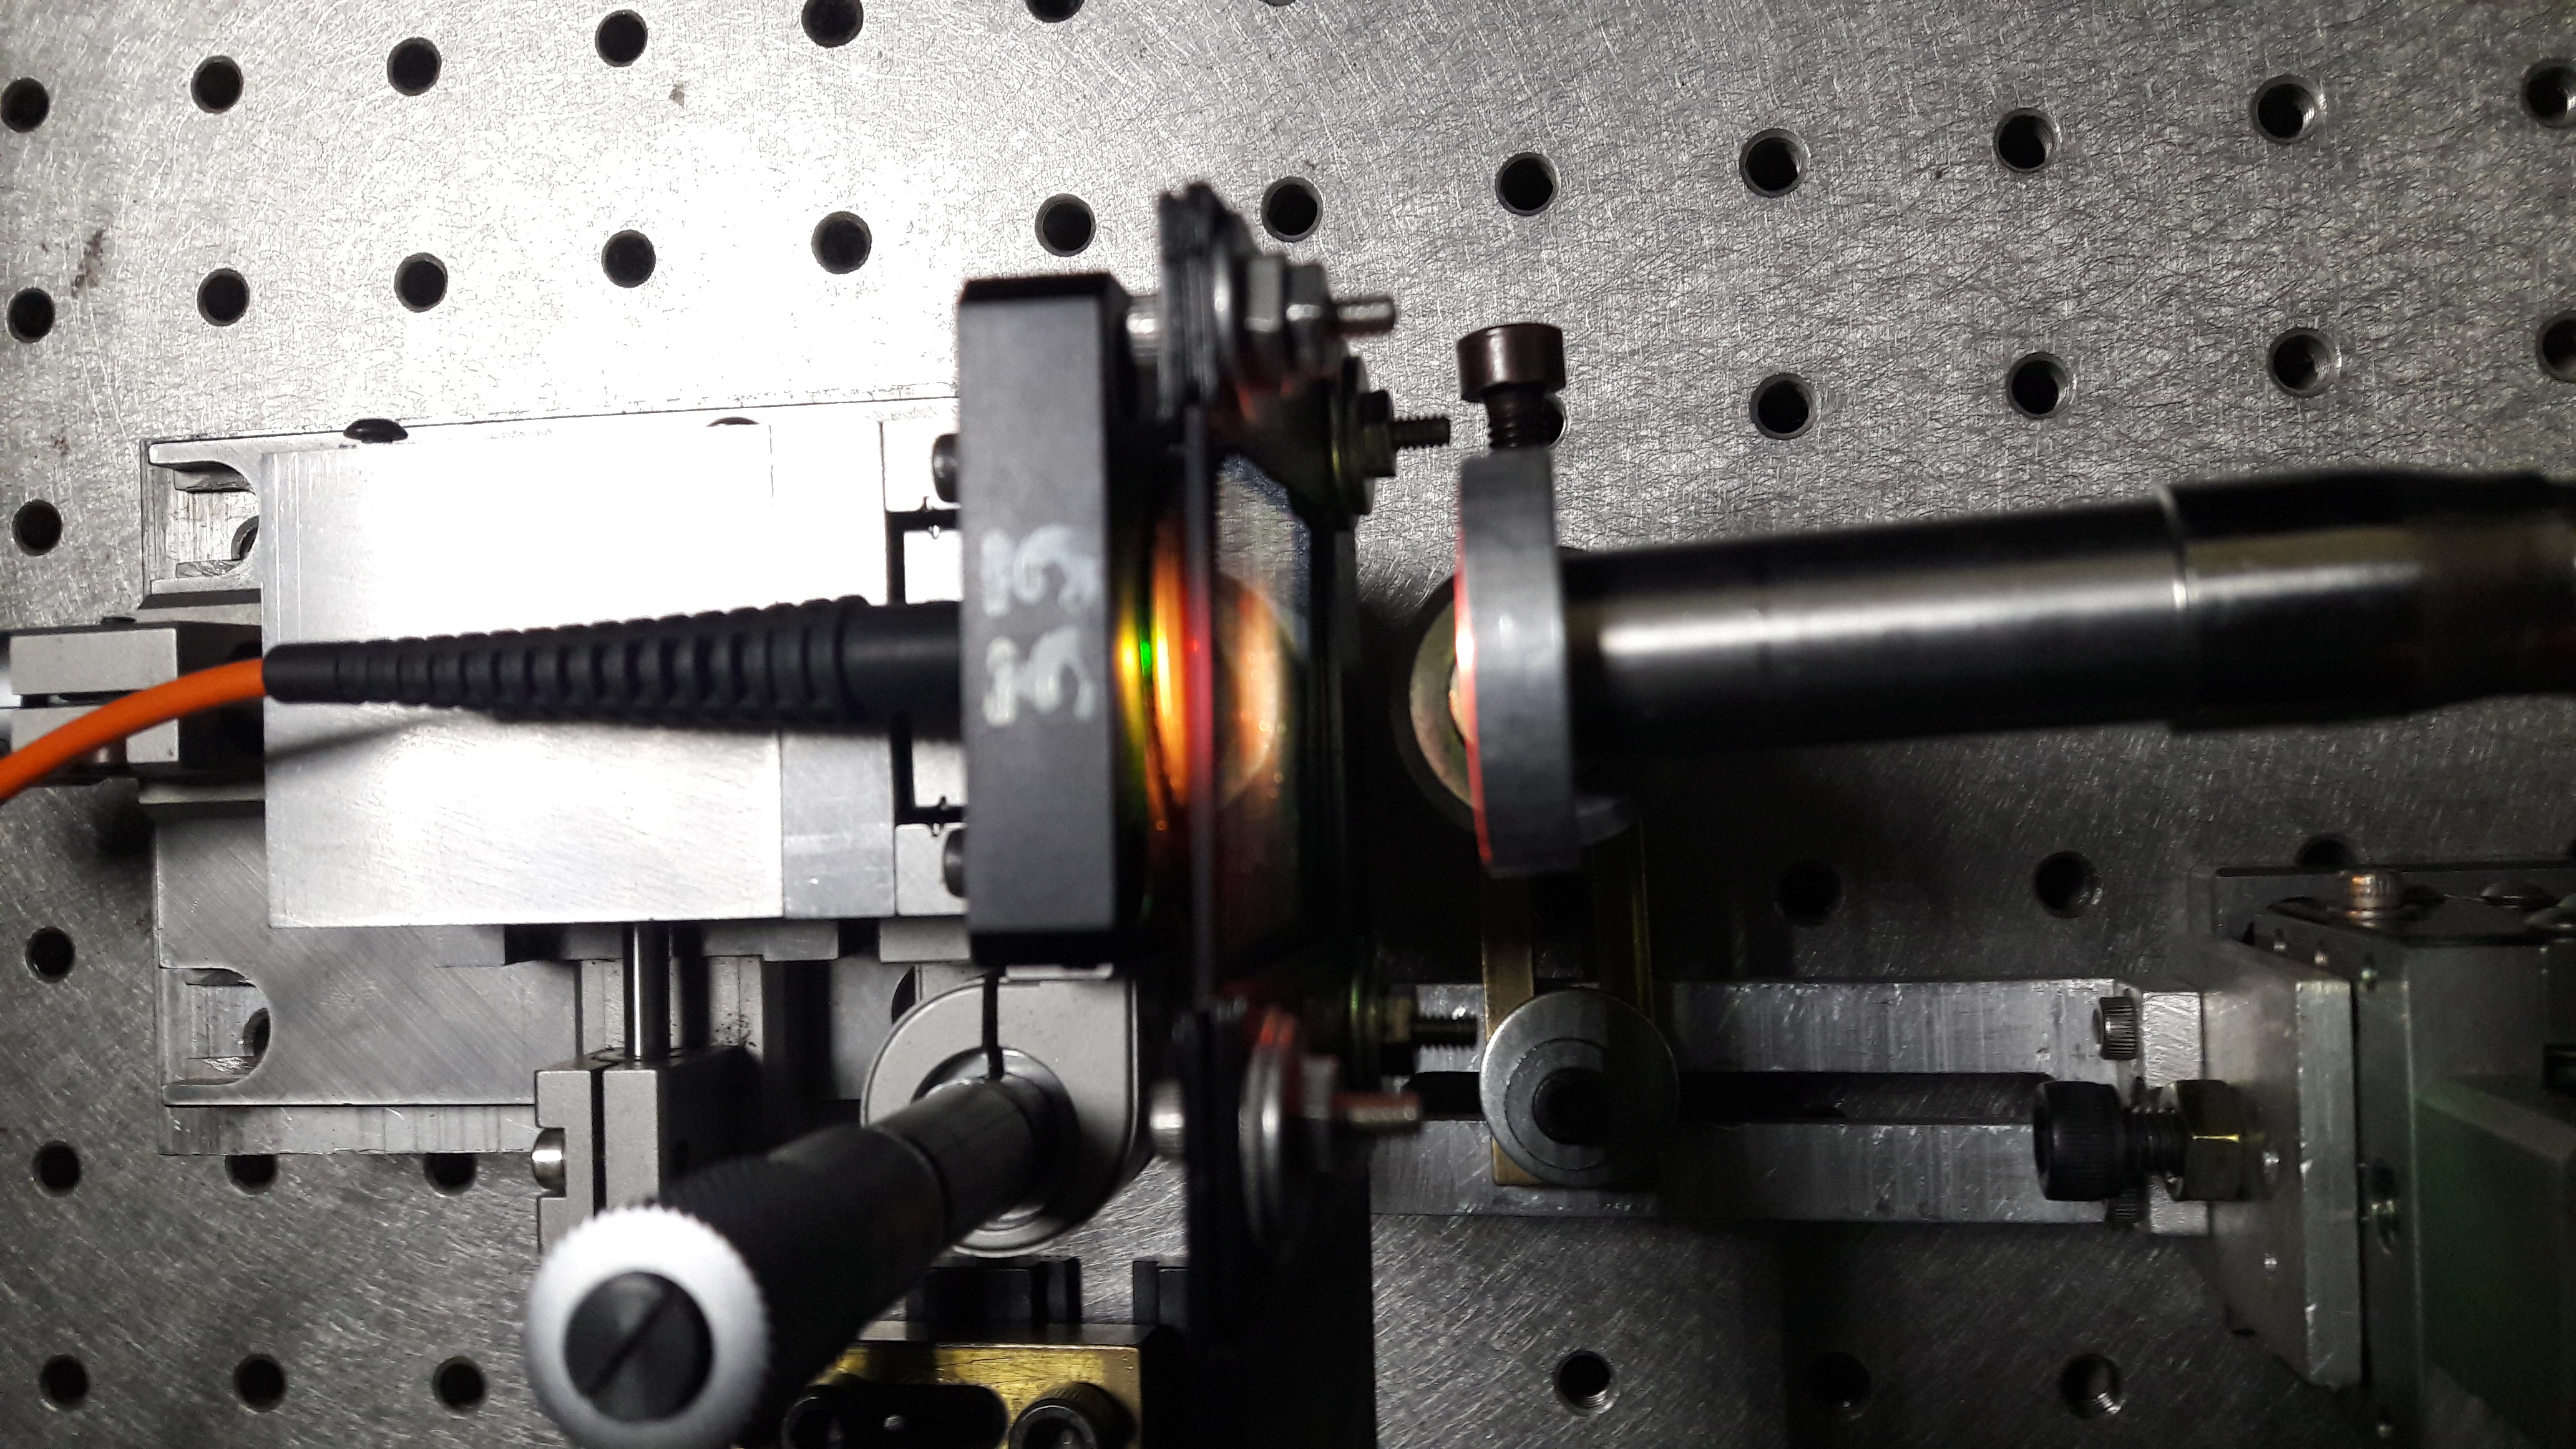
\includegraphics[scale=0.1]{imgs/setup_barrido/6.jpg}
\end{center}

\begin{center}
	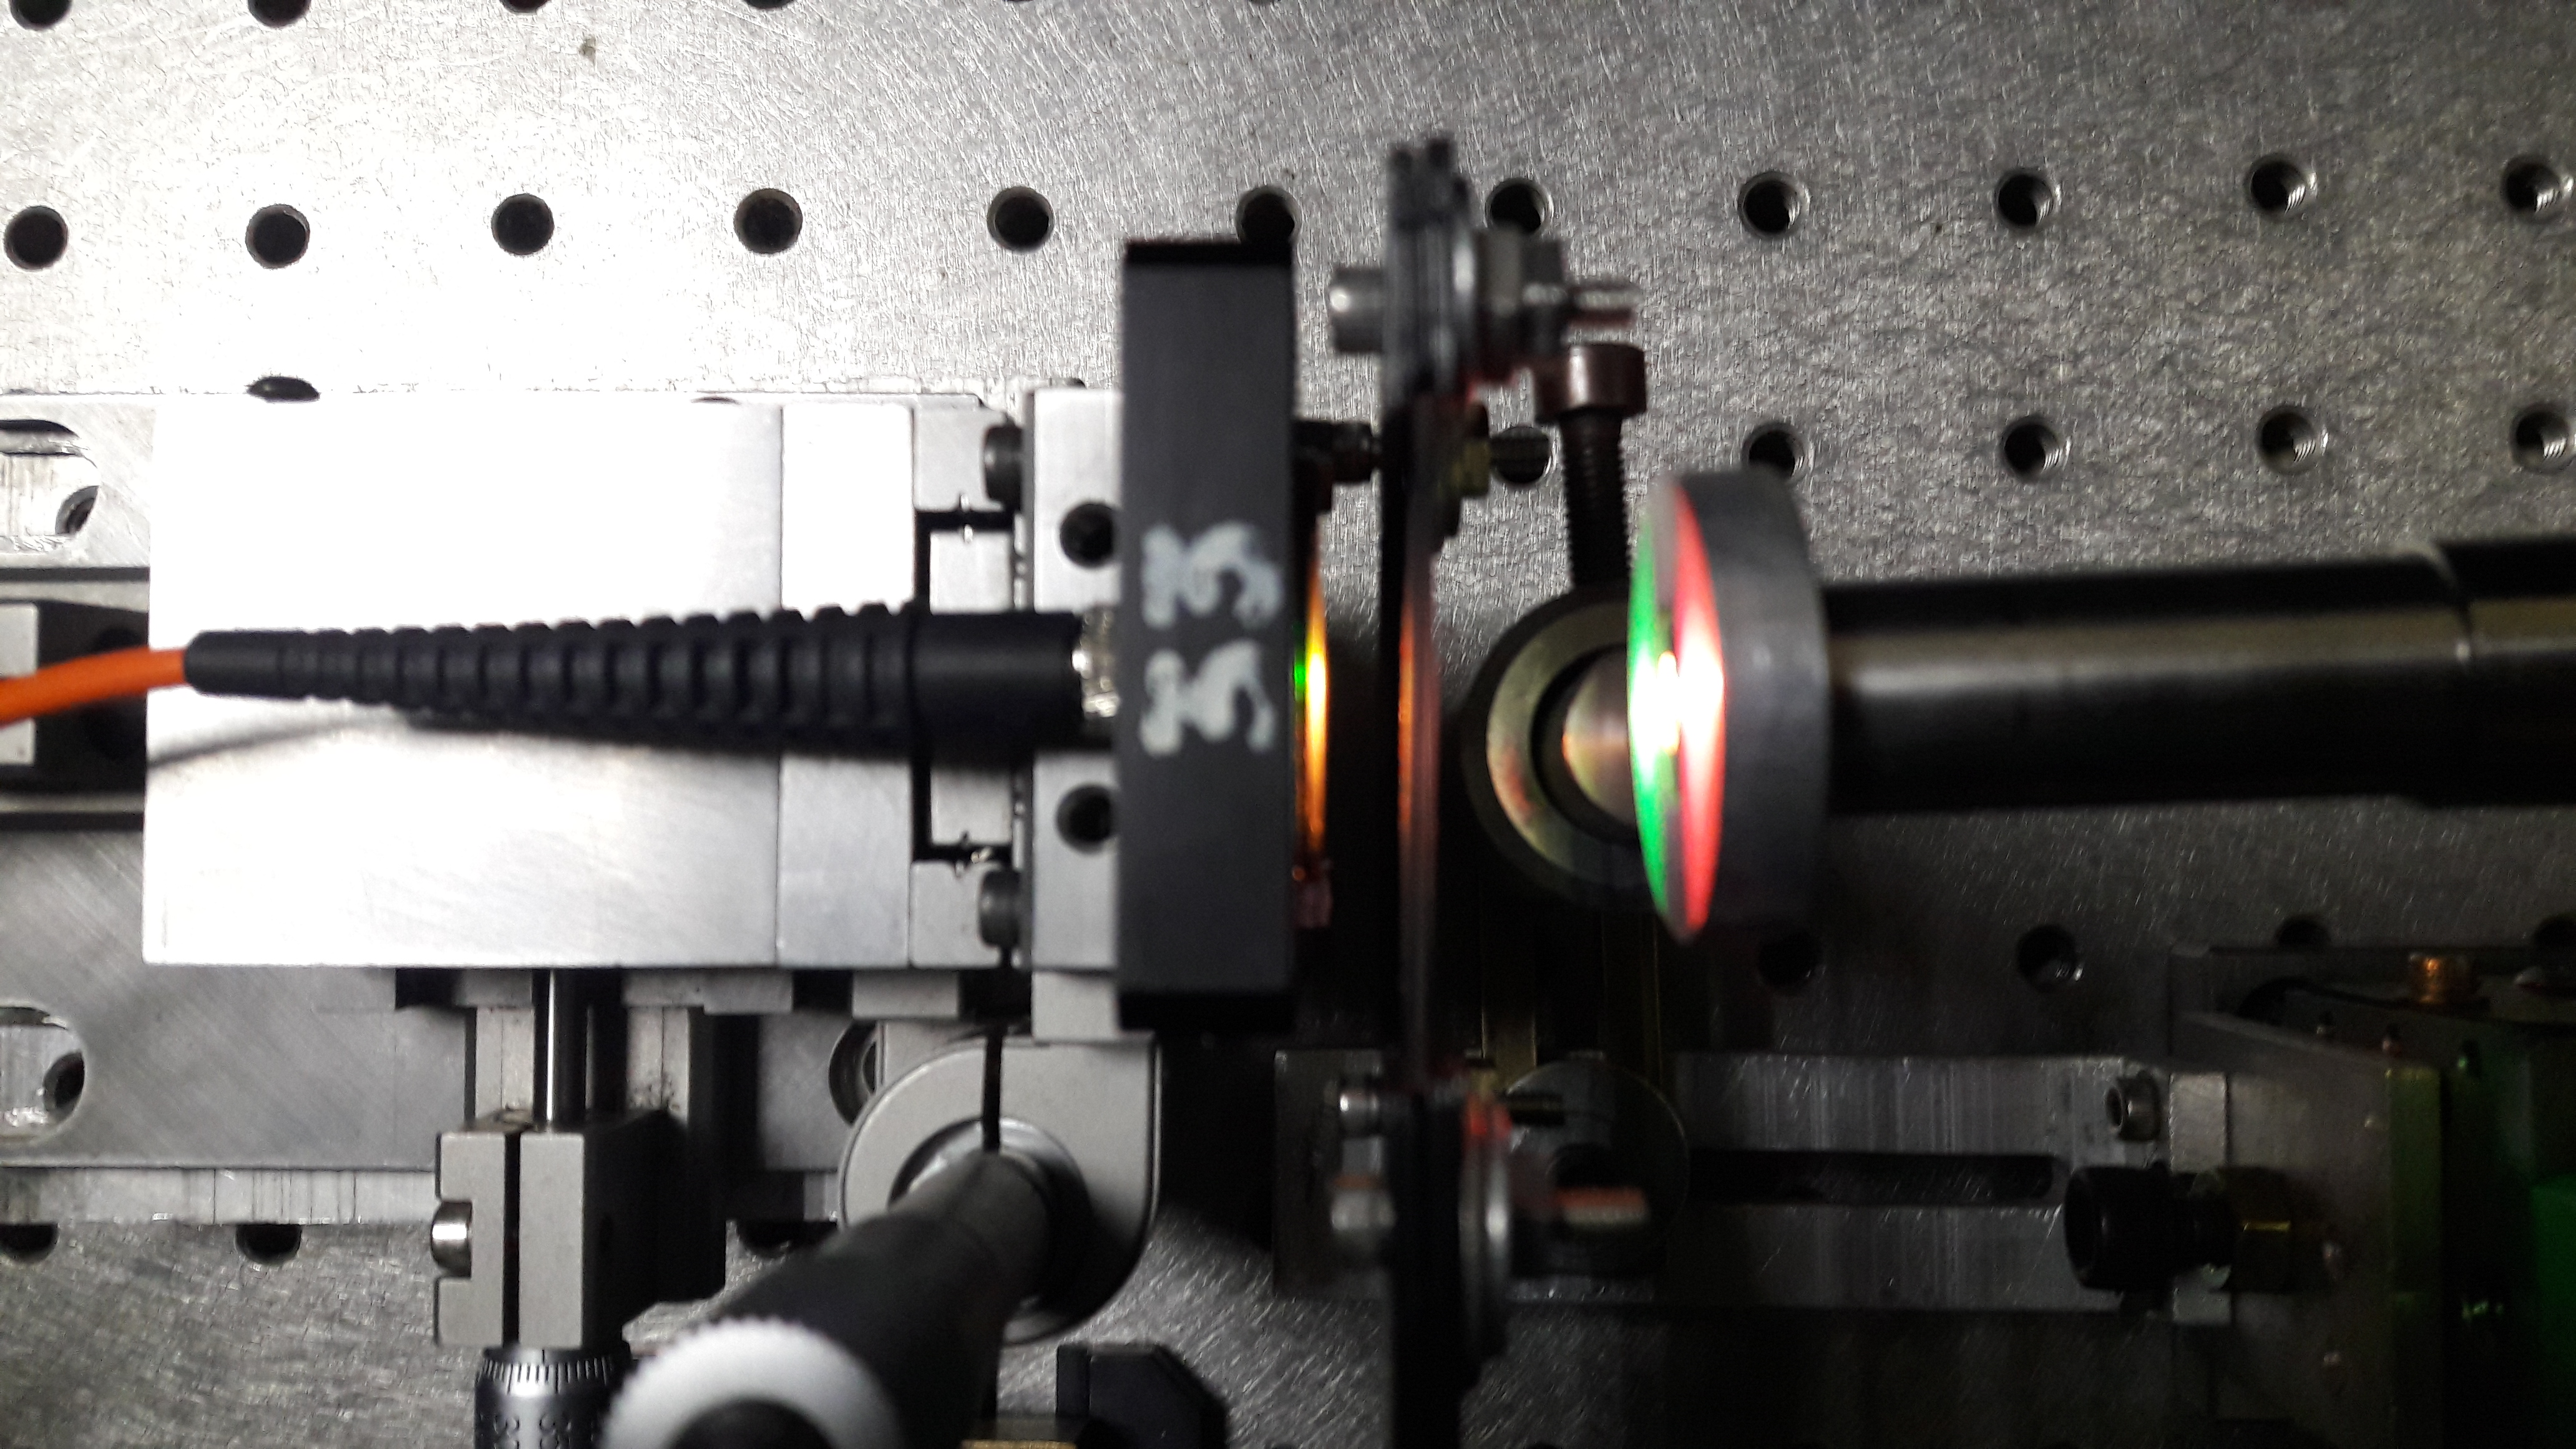
\includegraphics[scale=0.1]{imgs/setup_barrido/7.jpg}
\end{center}

\begin{center}
	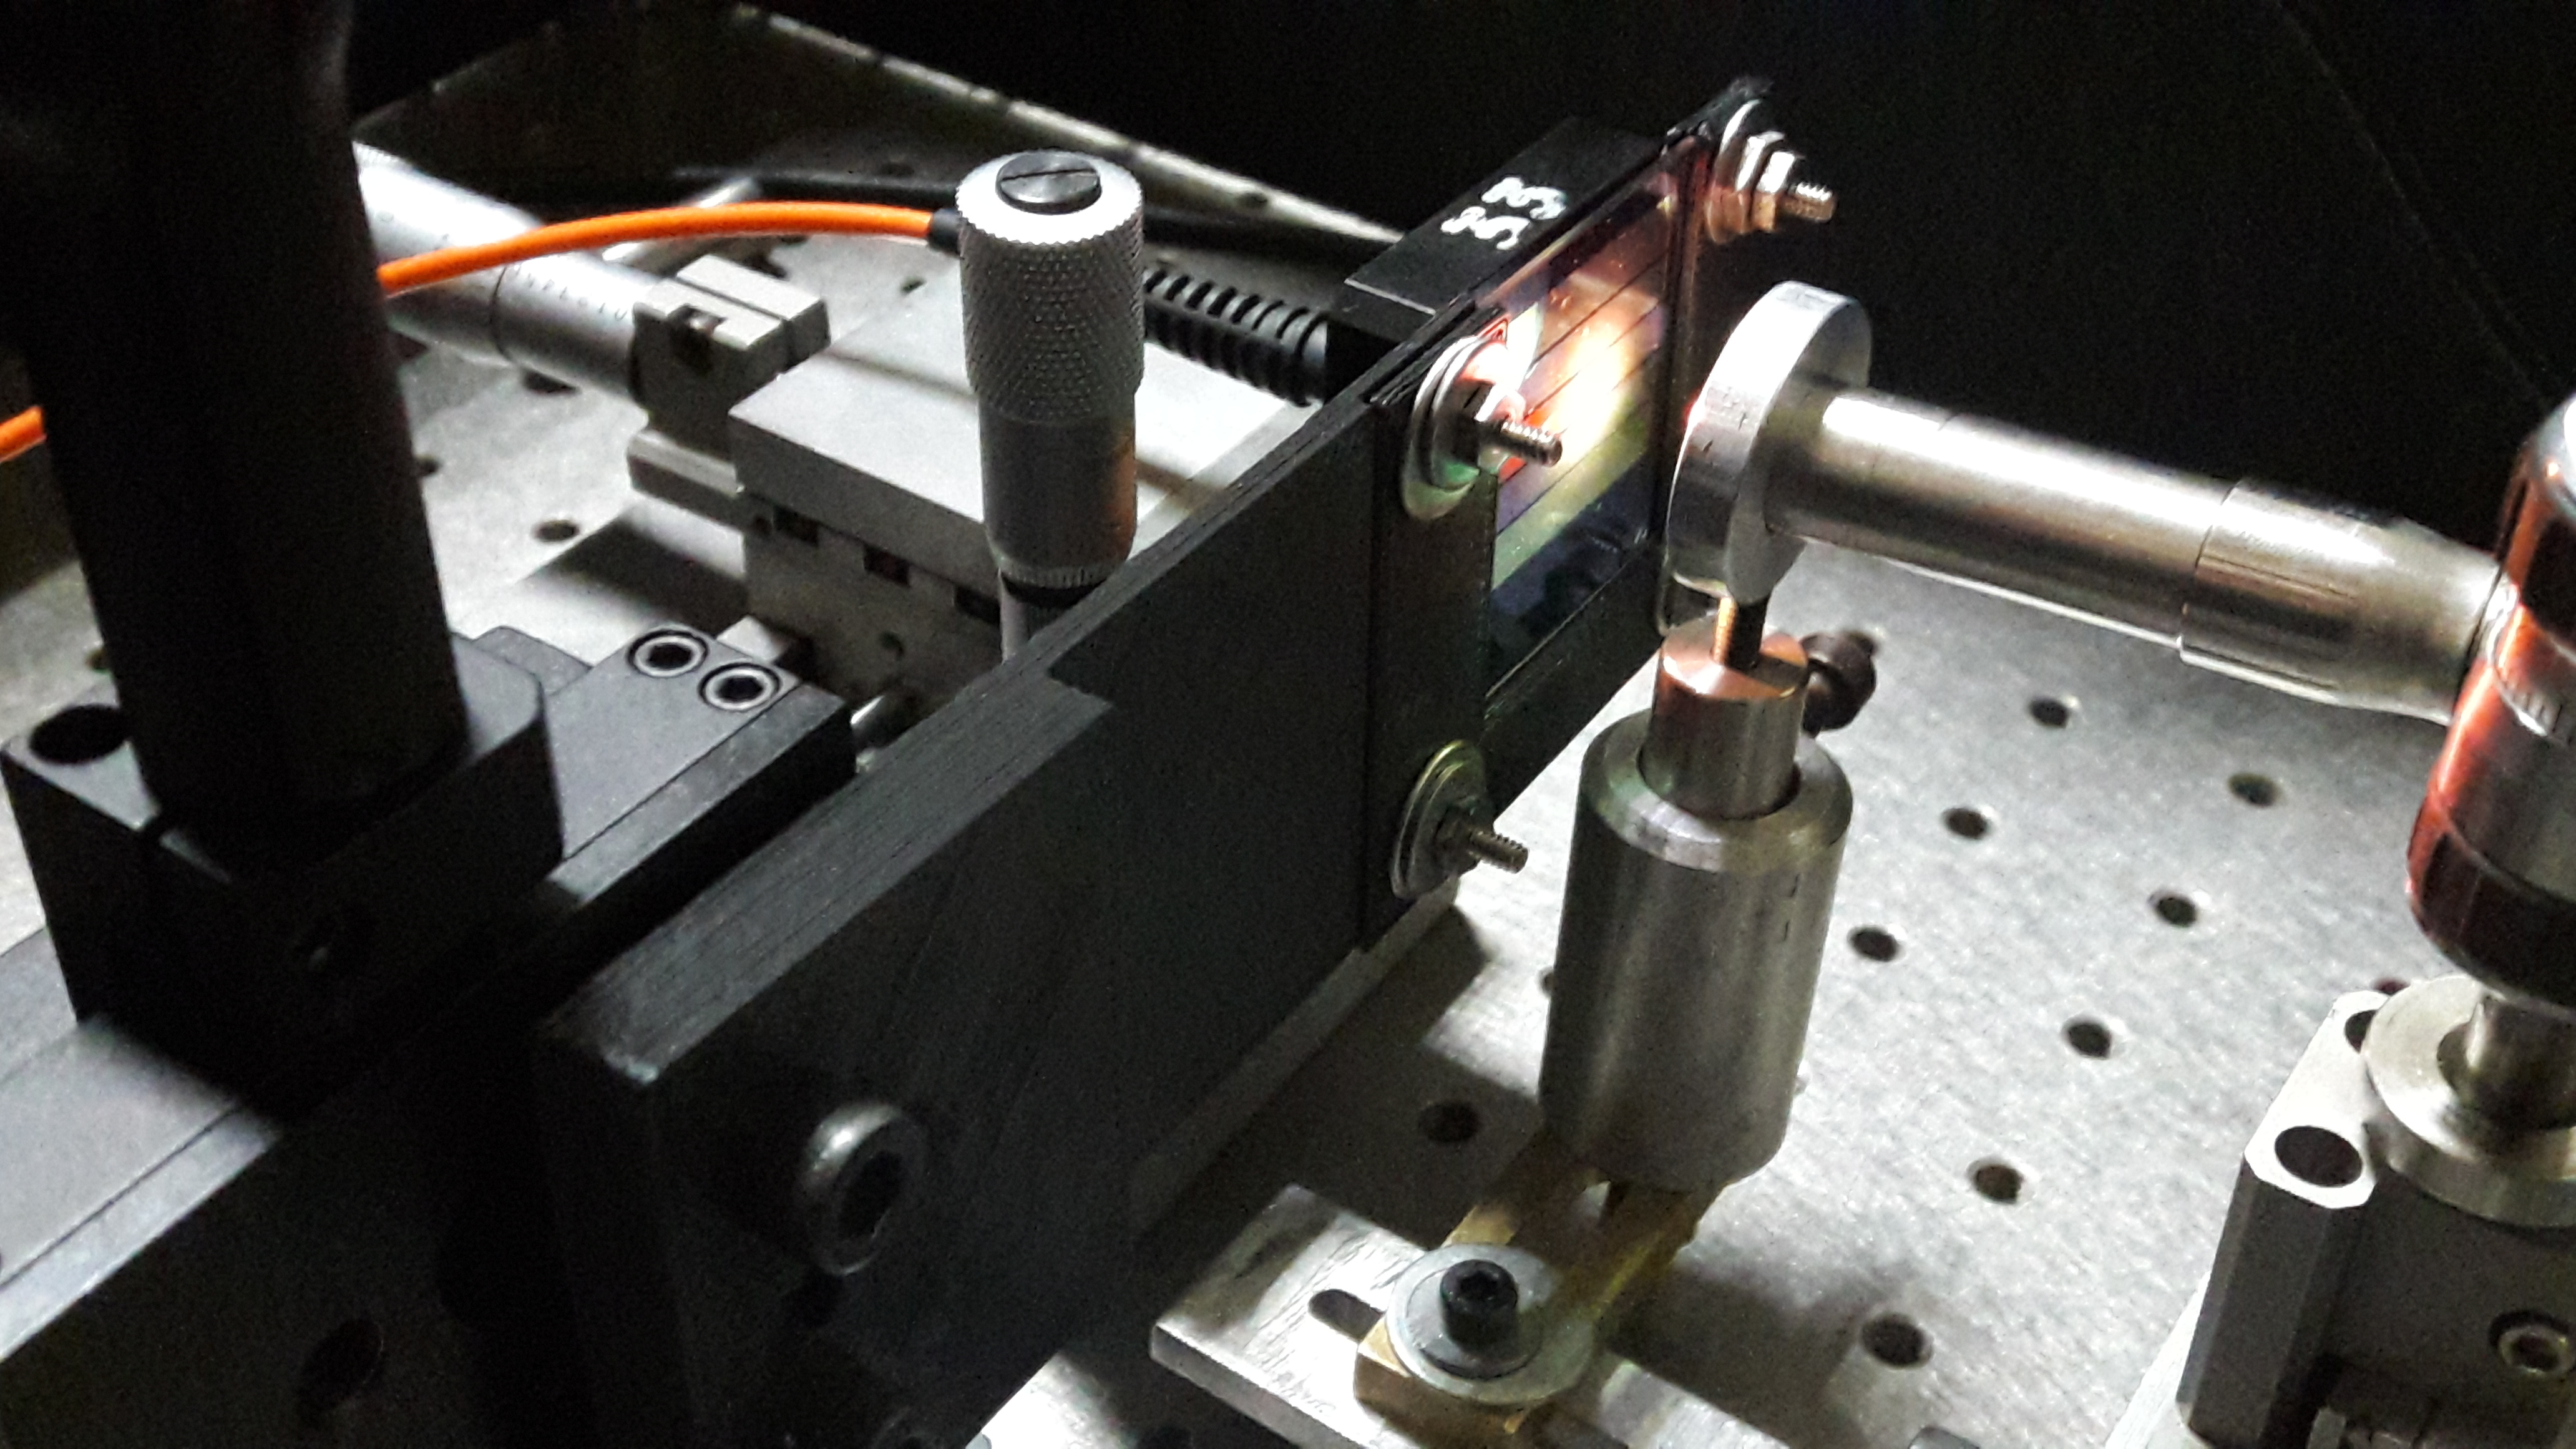
\includegraphics[scale=0.1]{imgs/setup_barrido/8.jpg}
\end{center}

\begin{center}
	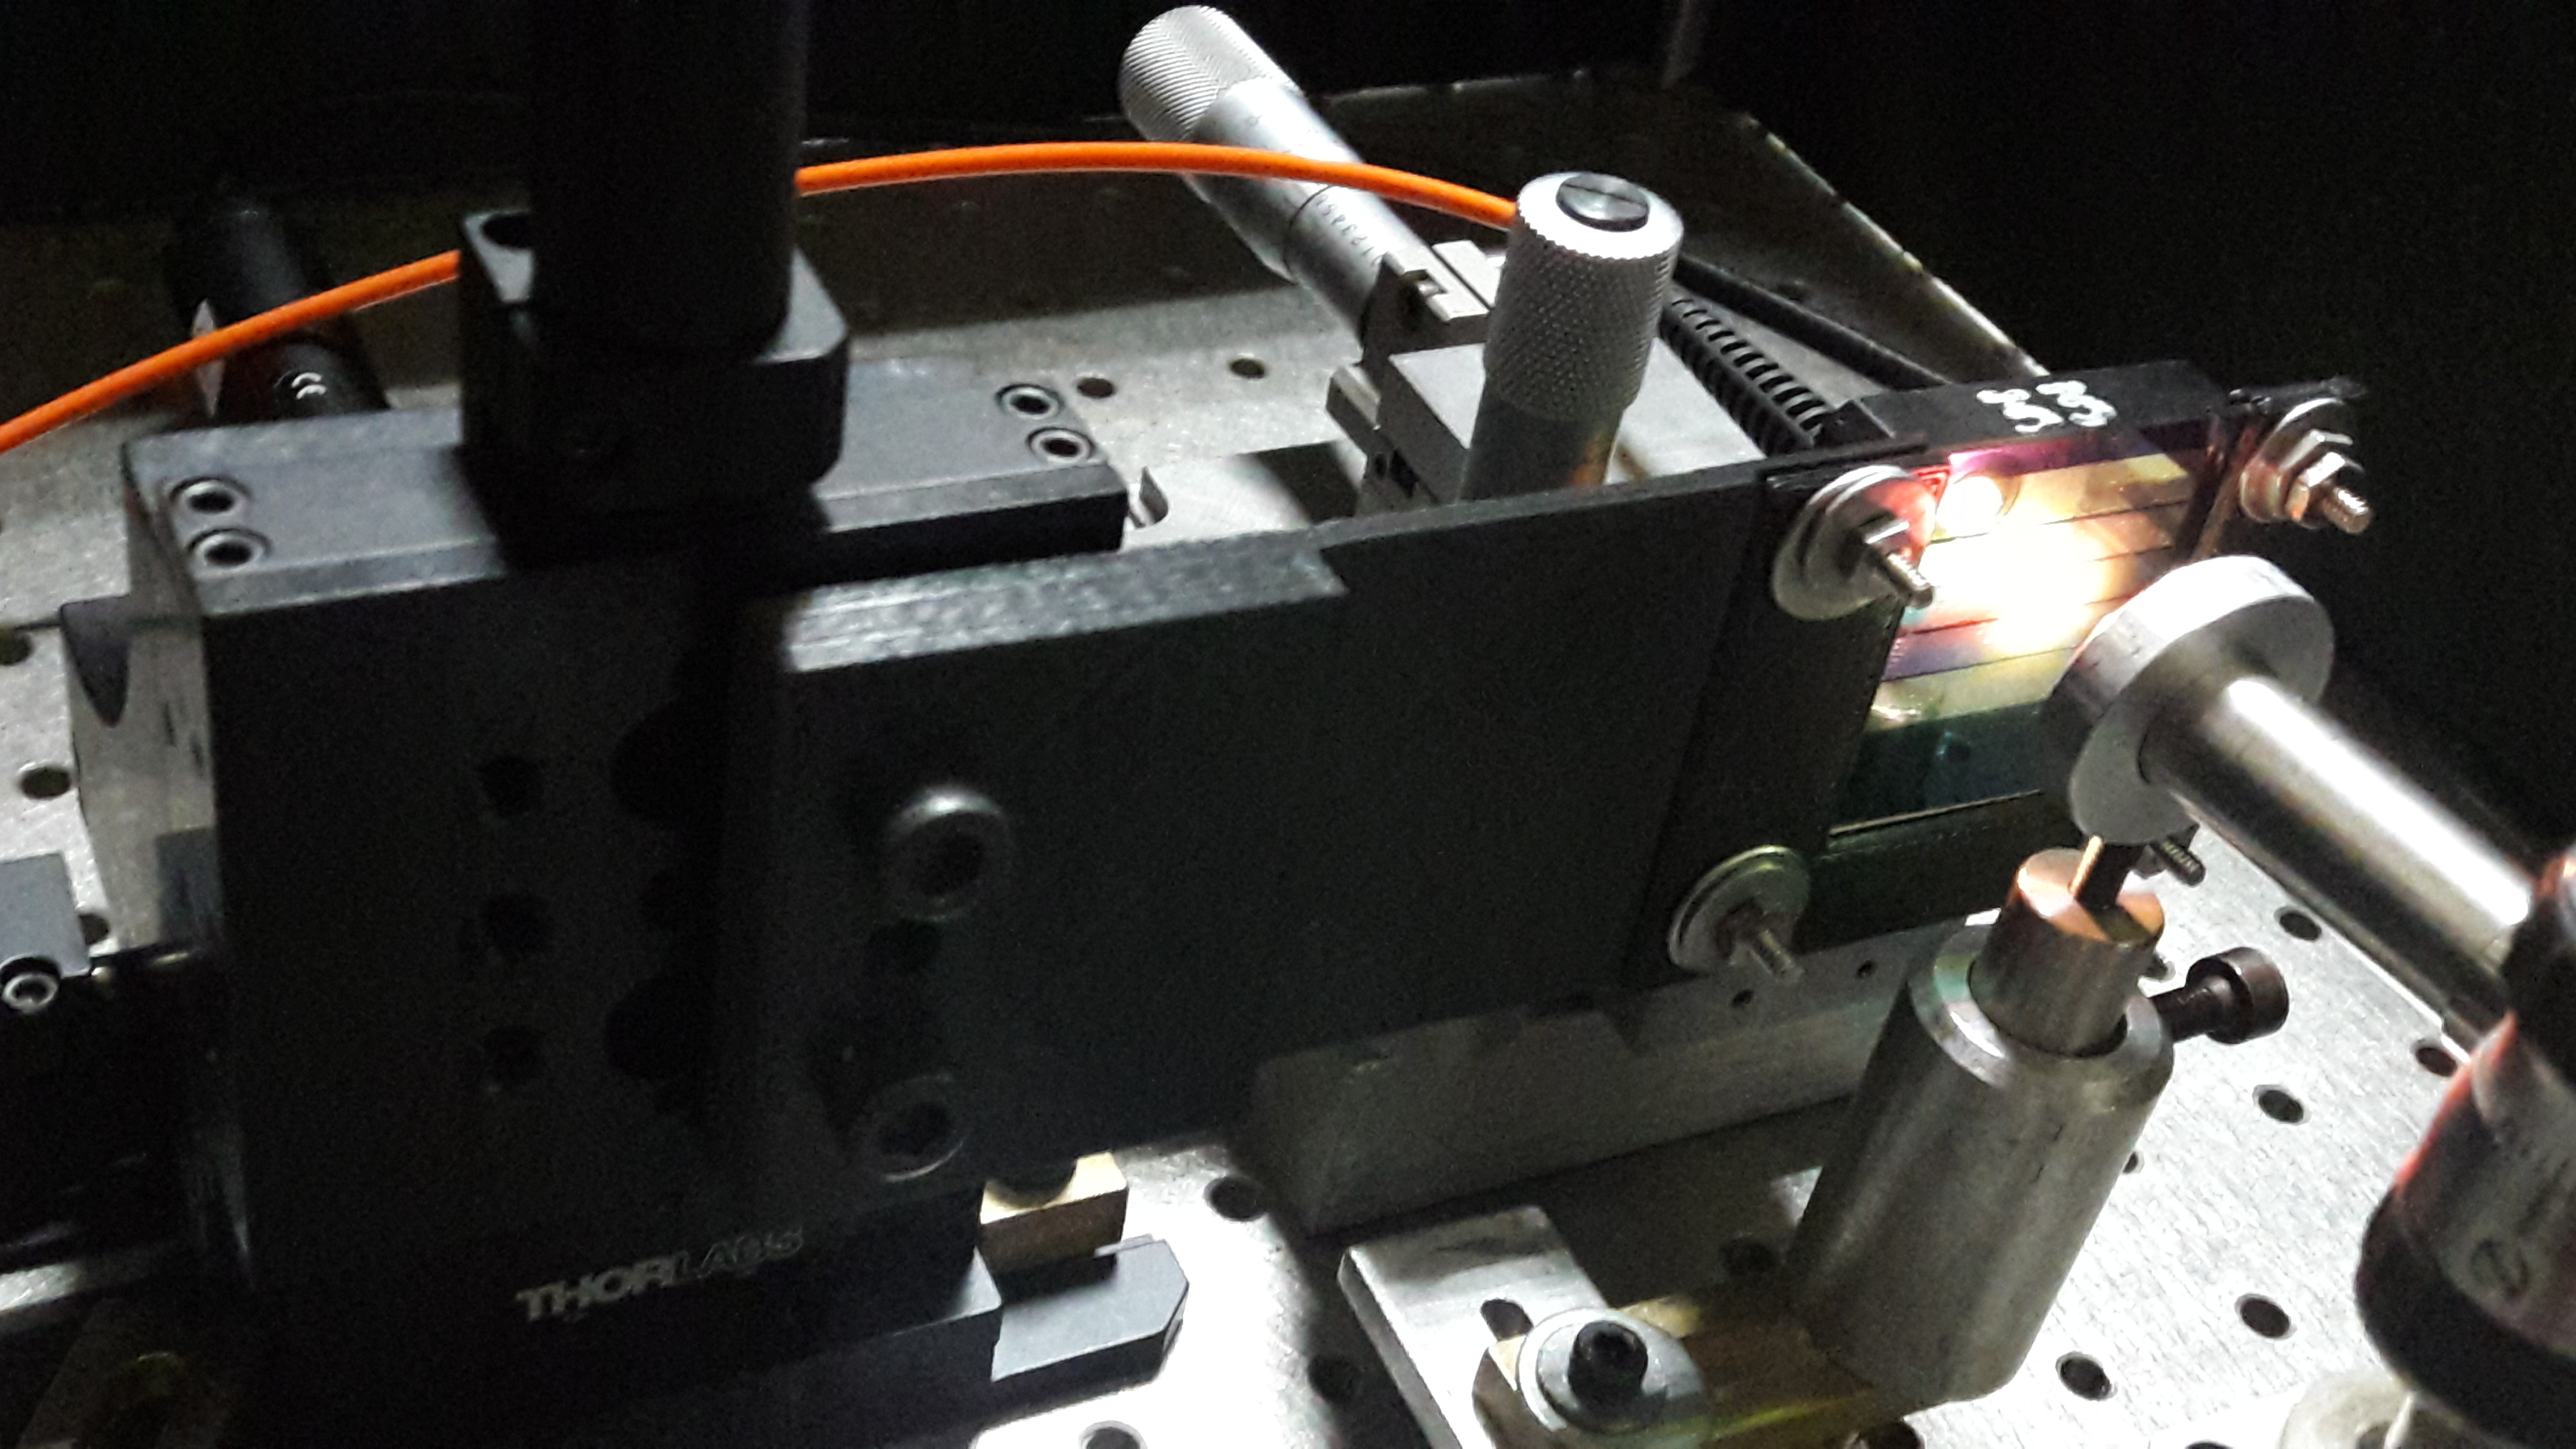
\includegraphics[scale=0.1]{imgs/setup_barrido/9.jpg}
\end{center}

\begin{center}
	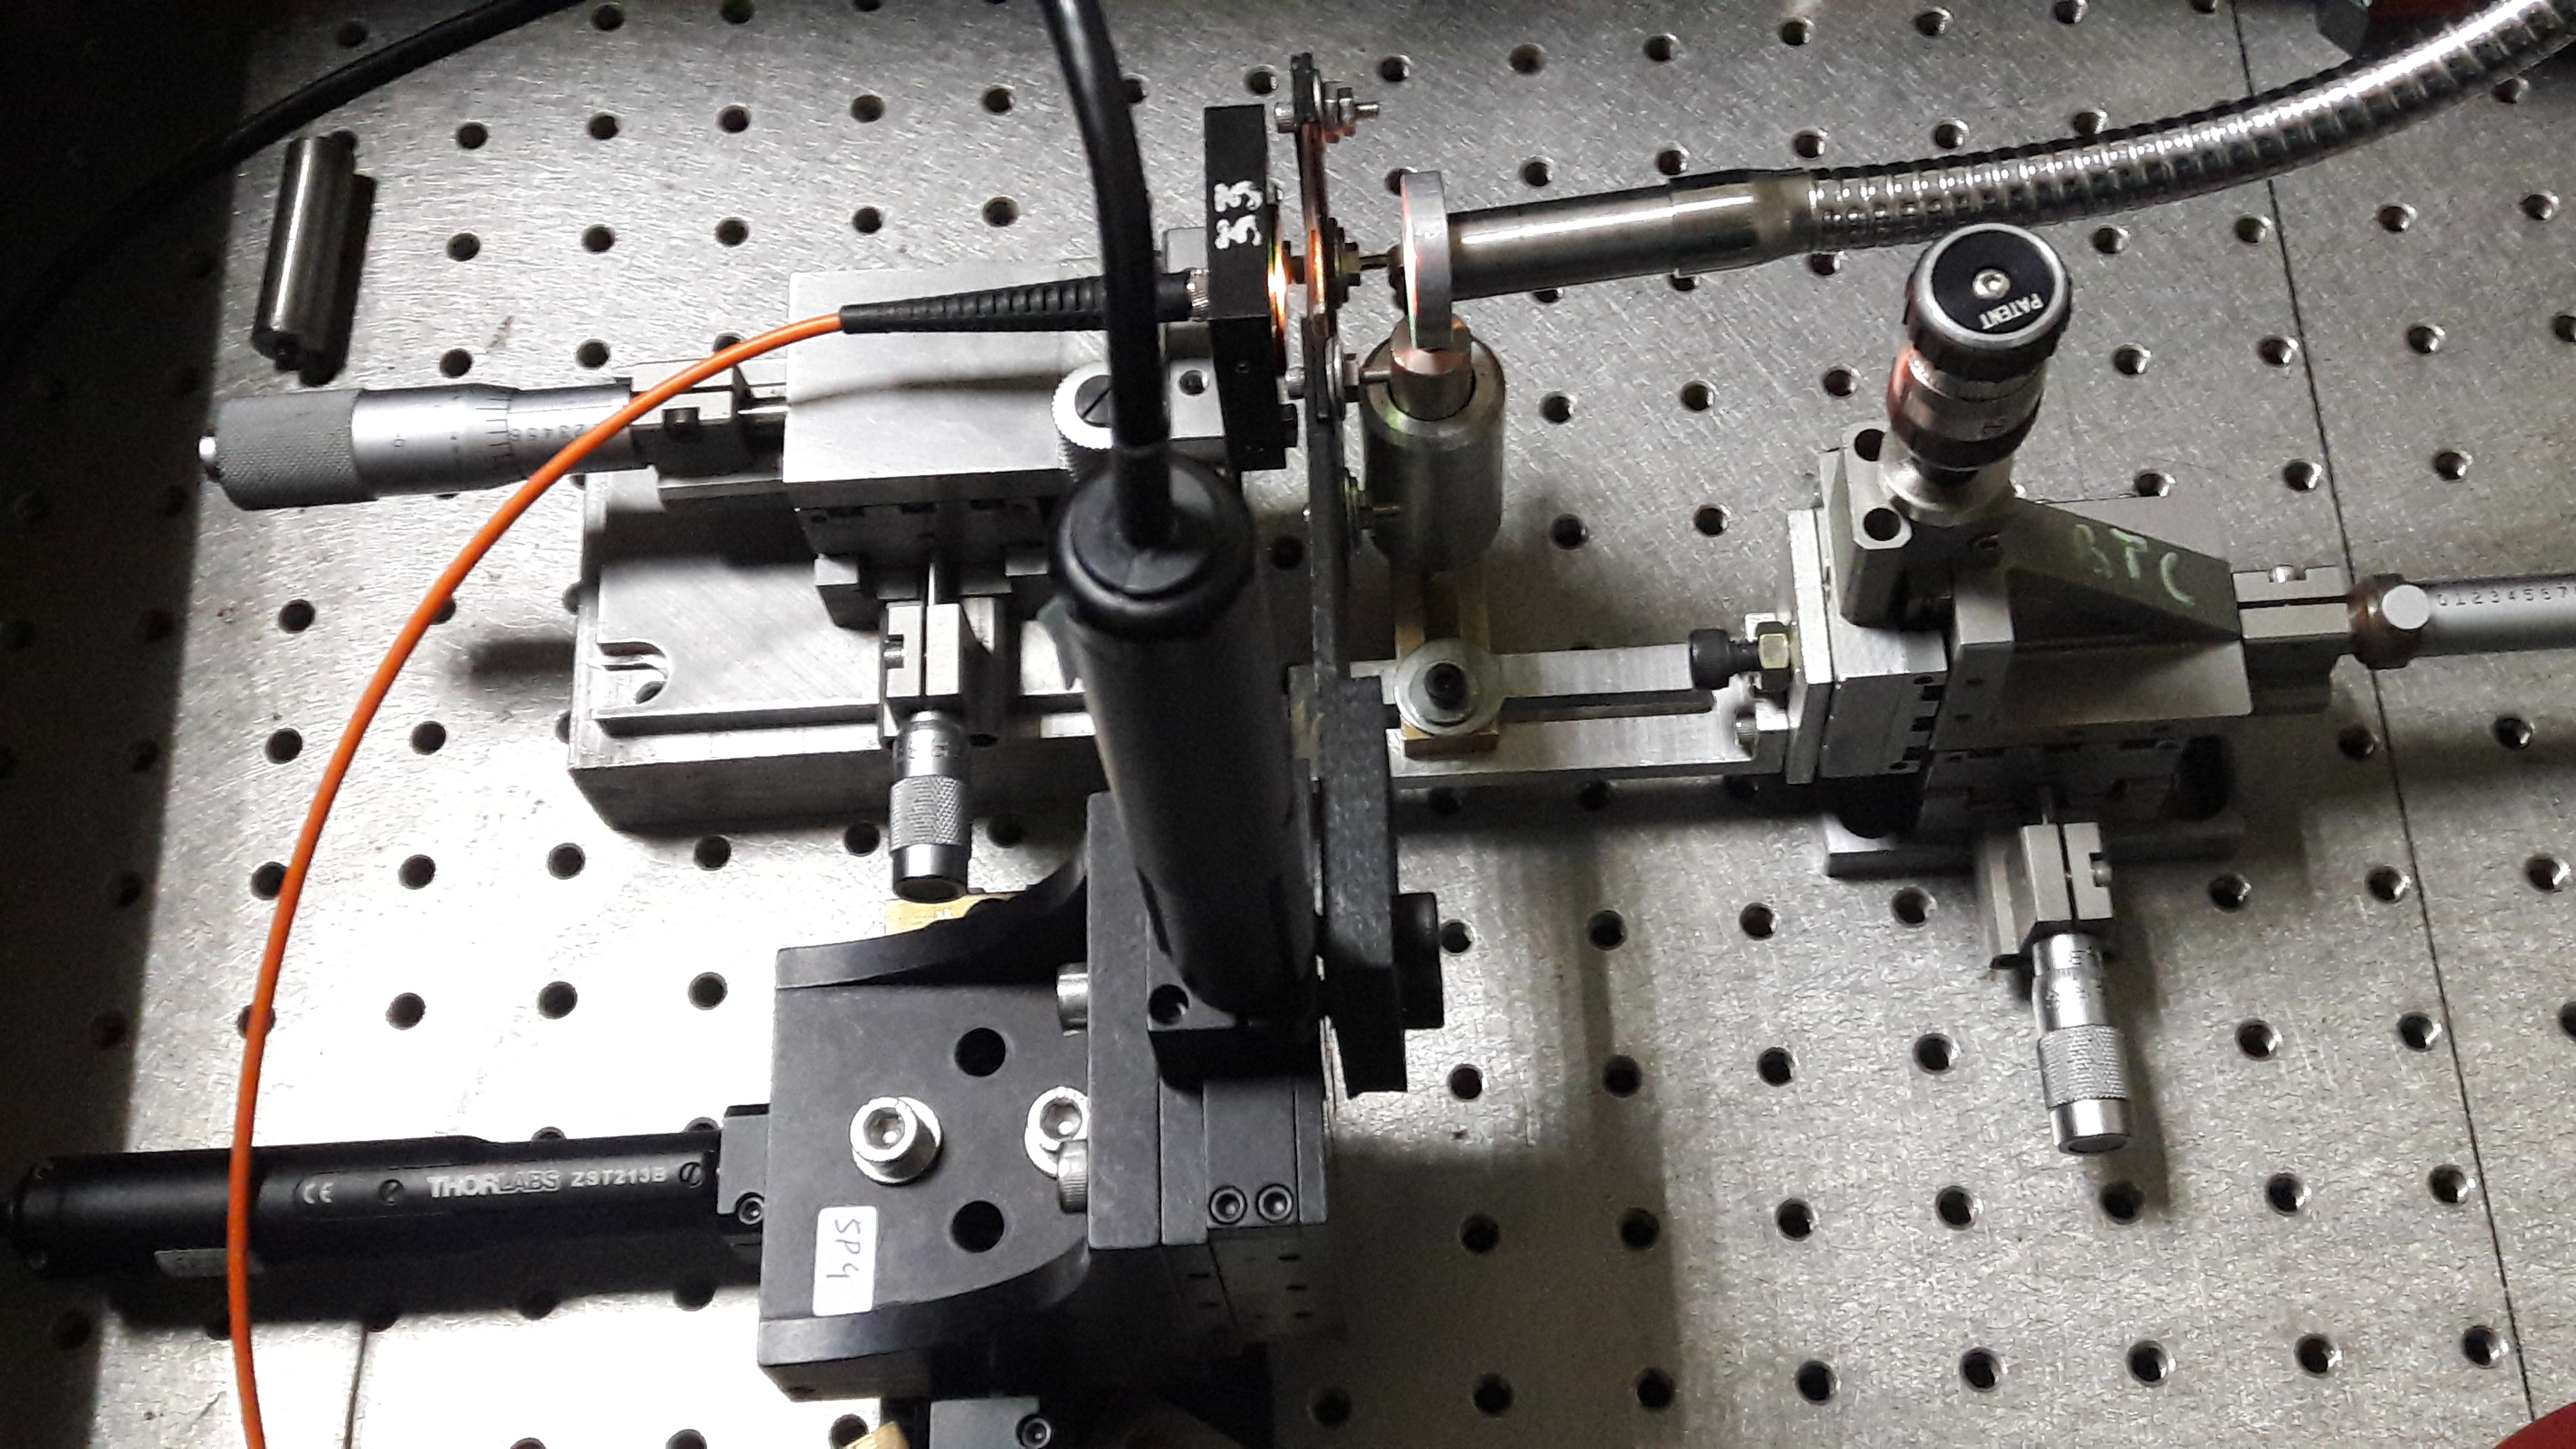
\includegraphics[scale=0.1]{imgs/setup_barrido/10.jpg}
\end{center}

\hrulefill

$2-8/10/2019$


 GUI - RGB.. zoom en las R-NIR bands.
\begin{center}
	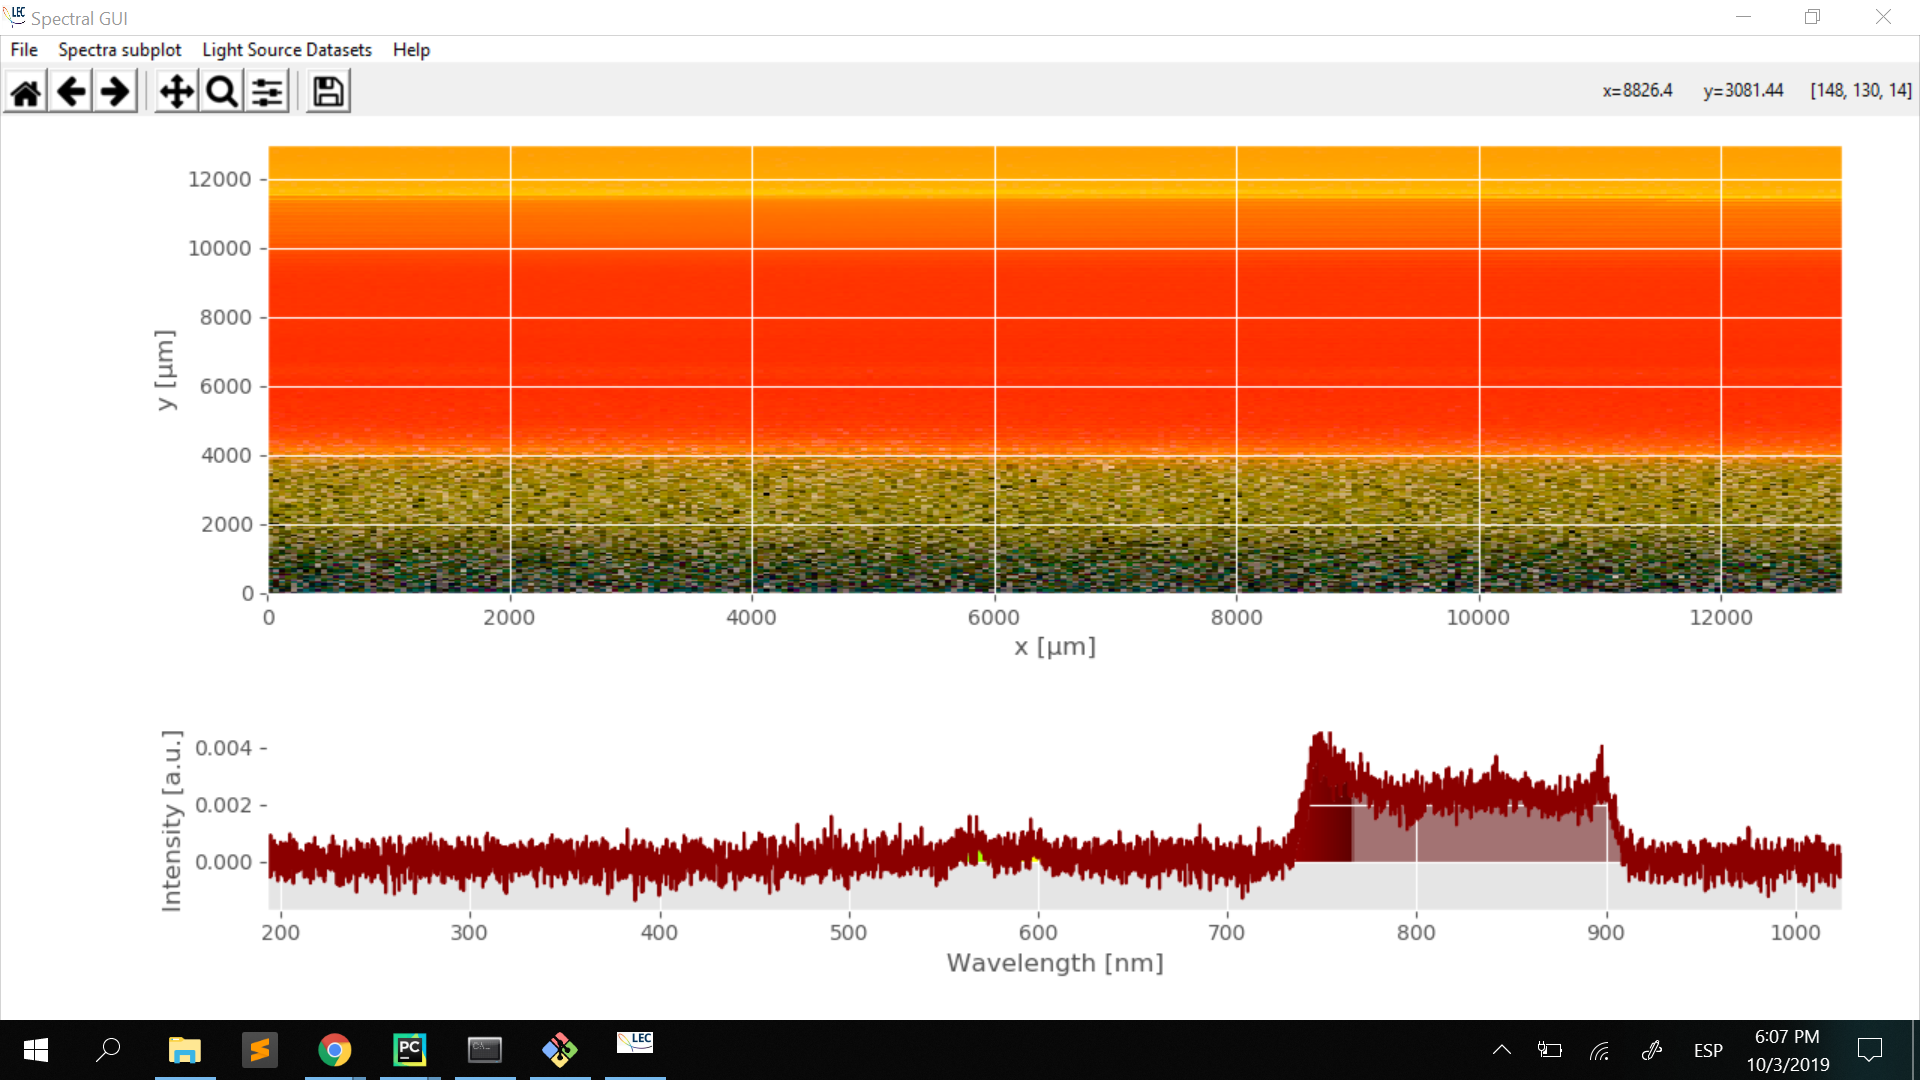
\includegraphics[scale=0.25]{imgs/gui/gui2.png}
\end{center}


\newpage
$RGB(x,y)_{band} - RGB^{mean}_{band}$:
\begin{center}
	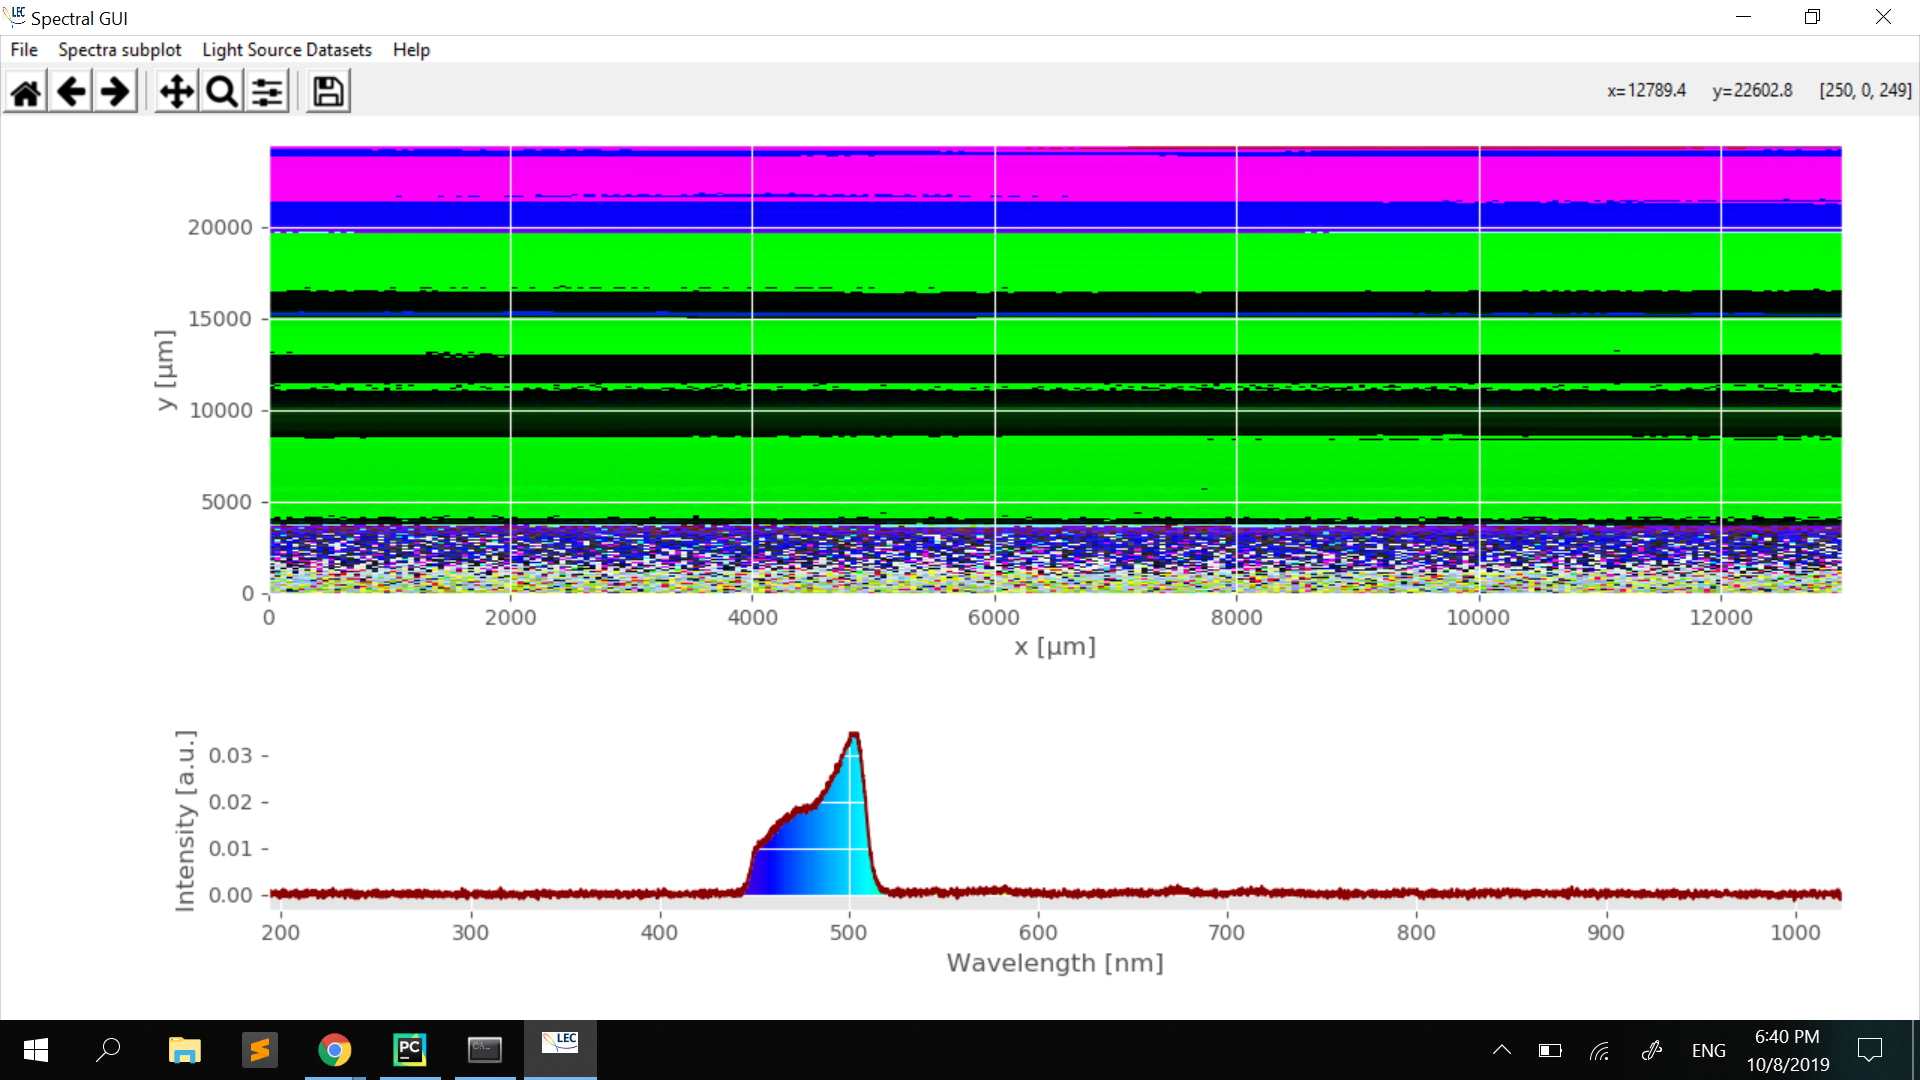
\includegraphics[scale=0.2]{imgs/gui/gui1.png}
\end{center}

obs: tiempos de integración/exposición distintos para la fuente y para el barrido filtro.



\hrulefill

$9/10/2019$

2D Motorized Stage incoming...


Some useful links:

\begin{itemize}
	\item \url{https://www.instructables.com/id/Motorized-Microscope-Stage-for-Olympus-IX50/}
	\item \url{https://www.sciencedirect.com/science/article/pii/S095656631631106X}
		\item \url{https://reader.elsevier.com/reader/sd/pii/S095656631631106X?token=CD853FD8472ADE524471296014E6F0B954A92E27109FDAE3938642B1E14D24881141960DA2FD9ABFE568803AC8D6CFE6}
\item \url{http://www.optics-focus.com/motorized-xy-microscope-stage-p-541.html#.XZ5TkEZKg2w}
	\item \url{https://www.thorlabs.com/newgrouppage9.cfm?objectgroup_id=5360&pn=MLS203-1}	
	\item \url{https://www.instructables.com/id/Internet-Arduino-Controlled-T-Slot-XY-Table/}
	\item \url{https://www.instructables.com/id/Low-cost-digital-microscope-with-automated-slide-m/}
\end{itemize}


Paper fundamental a seguir:
\href{https://reader.elsevier.com/reader/sd/pii/S095656631631106X?token=D9588CB30F54FB09F8EA5C89EB096F16036AD47E209DD10BCB3138EE9C6500AE62D6D0902D2BB257A30B763BE6C51B37}{LINK}


Presupuesto/Lista de ''materiales'':

\begin{enumerate}
	\item 16 piezas impresora 3D.
	\item Arduino \begin{itemize}
	
	\item Arduino Due $\xrightarrow{}$ \href{https://candy-ho.com/producto/arduino-due-r3-cable-usb-atsam3x8e-arm-cortex-m3-512-kb/}{$\sim$ \$1400}
	
	\item Arduino UNO $\xrightarrow{}$ \href{https://candy-ho.com/producto/arduino-uno-r3-cable-usb-domotica-robotica-atmel-original/}{$\sim$ \$750} 	
	\end{itemize}
	\item 2 motores paso a paso NEMA 17 - Modelo MKP42HT47-1684A $\xrightarrow{}$ \href{https://candy-ho.com/producto/motor-nema-17-alto-torque-0-9-4-4kg-impresora-3d-prusa-i3/}{$\sim$ \$1700 x 2} $\xrightarrow{}$ VER I (CURRENT) DEMAND -- FUENTE ATX? 
	
	En 3D insumos están \$200 más caros: \href{https://3dinsumos.com.ar/Producto/3DPrinter-Nema17-AltoTorque0.9}{LINK}

\item Varilla roscada de diámetro 8 mm de X HILOS (IMPORTANTE, determina el paso): que la varilla venga/comprar con la camisa + tuerca
\begin{itemize}
\item  $\sim$ \href{https://candy-ho.com/producto/varilla-rosca-husillo-ctornillo-prusa-reprap-8mm-400mm/}{\$800 x 2 en CANDY-HO} (aparente' no es de 4 hilos, es de 1 hilo entonces avanza 1mm por cada 'firulete', con 4 hilos avanza mucho más rápido (paso + grande: con 1 vuelta de 4 hilos, se avanzan 8 mm))
\item $\sim$ \href{https://3dinsumos.com.ar/Producto/3D-VarillaRoscadaM8}{\$ 200 x 2 en 3D INSUMOS} 
\end{itemize}

\item Acoples flexibles de 5mm (diametro del eje del nema 17 (\texttt{shaft diameter})) a 8mm (diámetro de la varilla roscada) x 2 $\xrightarrow{}$ $\sim$ \href{https://3dinsumos.com.ar/Producto/3DPrinter-AcopleAlu5-8}{\$ 150 x 2 en 3D INSUMOS}
\item 4 Ejes de acero de 8mm de diámetro, x mm de largo $\xrightarrow{}$ \href{https://3dinsumos.com.ar/Producto/3DPrinter-Varilla8mmX320mm}{\$ 300 x 4 ( 2 para cada DoF)}
\item 4 rodamientos que van sobre los ejes de acero $\xrightarrow{}$ \href{https://3dinsumos.com.ar/Producto/3DPrinter-Rul-SCS8UU-ConSoporte}{\$ 450 x 4 ( 1 para cada eje)}
\item \texttt{ball bearings} (rulemanes, ó rodamientos, hay en 3D INSUMOS)
\item \texttt{four M4 brass guide rods.}
\item 4 end switches - 2 para x - 2 para y
\item \texttt{65 standard M2-4 screws and
nuts.}
	\item Controlador: \begin{itemize}
\item Puente H L293DNE en un shield montado arriba del arduino UNO.
\item 	Driver LV8729 hasta 1/128 micropasos 1.5A Max $\xrightarrow{}$ \href{https://3dinsumos.com.ar/Producto/3DPrinter-DriverLV8729}{$\sim$ \$800 x 2}
	\end{itemize}
\end{enumerate}

\newpage

\hrulefill

$15/10/2019$


Eje x:

\begin{center}
	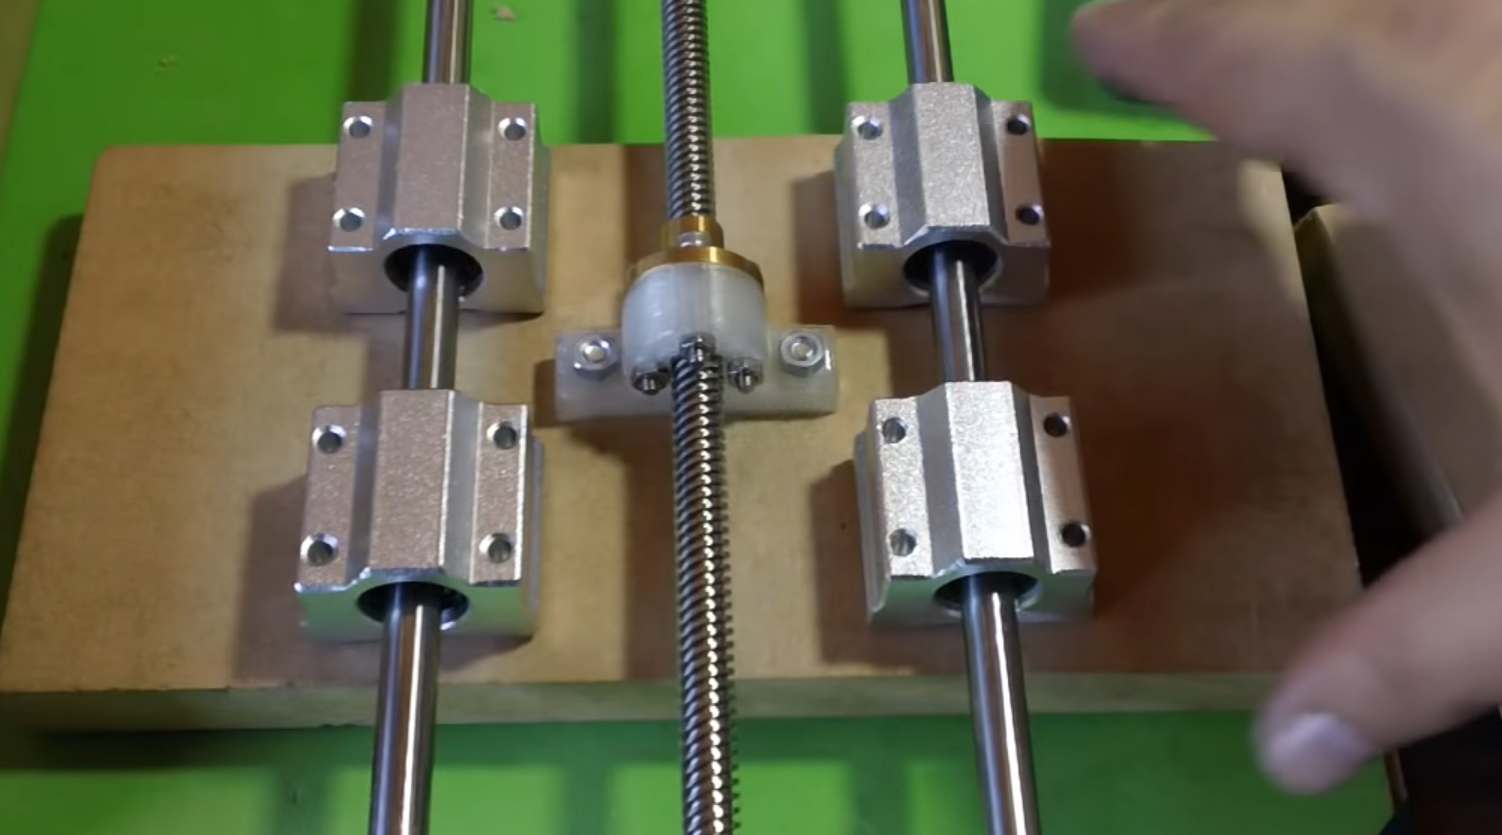
\includegraphics[scale=0.8]{imgs/eje_x.png}
\end{center}

\hrulefill

$17/10/2019$

\begin{center}
	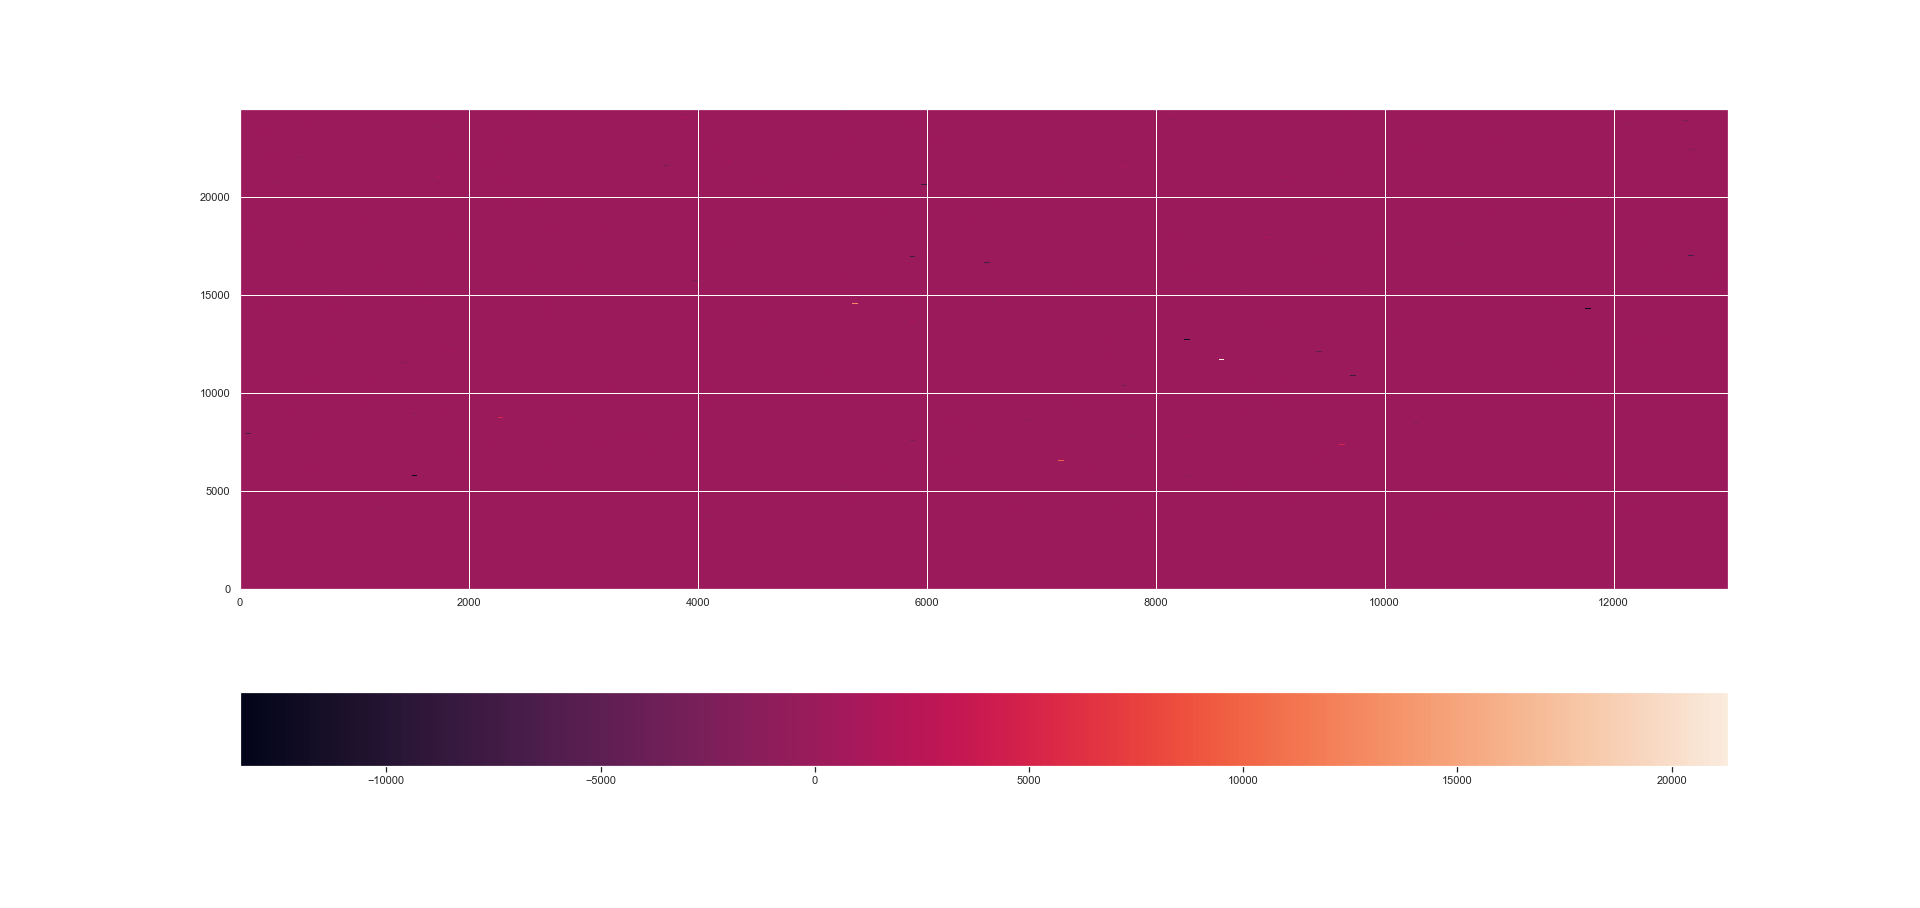
\includegraphics[scale=0.3]{imgs/gui/chi_sq.png}
\end{center}

\begin{center}
	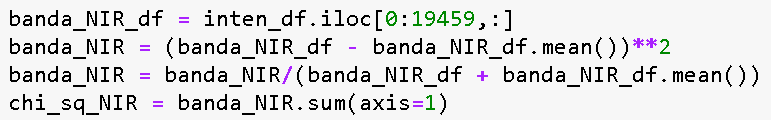
\includegraphics[scale=1.0]{imgs/gui/chunk_sq.png}
\end{center}


\end{document}
